\documentclass{article}

\usepackage{amssymb}
\usepackage[polish]{babel}
\usepackage[utf8]{inputenc}
\usepackage{polski}
\usepackage{geometry}
\usepackage{graphicx}
\usepackage[T1]{fontenc}
\usepackage{lmodern,cmap}

\usepackage[none]{hyphenat}

\geometry{
	a4paper,
	left=30mm,
	right=30mm,
	top=30mm,
	bottom=25mm
}


\usepackage{amsmath}
\DeclareMathOperator{\sgn}{sgn}

\usepackage{pgfplots}
\pgfplotsset{compat=1.17}

\graphicspath{ {./images/} }
\usepackage{lipsum}
\usepackage{caption}
\usepackage{float}

\title{Klasyfikacja COVID-19 na zdjęciach rentgenowskich}
\author{Vladyslav Diachuk s18901}

\bibliographystyle{plain}

\makeindex
\begin{document}
%\pagenumbering{gobble}
\begin{titlepage}          
	\sffamily                                                                              
	
\includegraphics[width=\textwidth]{pjwstk_logo}

	\vspace{1.4cm}
	
	\begin{center}
		{
			\Large
			\textbf{Wydział Informatyki}
			\vspace{1.4cm}
			
			\textbf{Katedra Systemów Inteligentnych i Data Science}
			\vspace{0.5cm}
			
			Inteligentne systemy przetwarzania danych
			\vspace{1.4cm}
			
			\textbf{Vladyslav Diachuk}\\
			s18901
		}
		\vspace{1.2cm}
		
		{\huge\textbf{Klasyfikacja COVID-19 na zdjęciach rentgenowskich}}
	\end{center}
	\vspace{2cm}
	
	\begin{flushright}
		\Large
		Praca inżynierska\\	
		\vspace{0.4cm}	
		Piotr Gnyś
	\end{flushright}
	\vspace{3cm}
	
	\begin{center}
		\Large
		Warszawa, 02, 2022
	\end{center}
	
\end{titlepage}

\begin{titlepage}          
	\sffamily                                                                              
	
\includegraphics[width=\textwidth]{pjwstk_logo_en}
	
	\vspace{1.4cm}
	
	\begin{center}
		{
			\Large
			\textbf{Faculty of computer science}
			\vspace{1.4cm}
			
			\textbf{Intelligent data processing systems and Data Science}
			\vspace{0.5cm}
			
			Intelligent data processing systems
			\vspace{1.4cm}
			
			\textbf{Vladyslav Diachuk}\\
			s18901
		}
		\vspace{1.2cm}
		
		{\huge\textbf{Classification of COVID-19 in X-ray images}}
	\end{center}
	\vspace{2cm}
	
	\begin{flushright}
		\Large
		Engineering thesis\\	
		\vspace{0.4cm}	
		Piotr Gnyś
	\end{flushright}
	\vspace{3cm}
	
	\begin{center}
		\Large
		Warsaw, 02, 2022
	\end{center}
	
\end{titlepage}

%===================================================================================
\section{Wstęp}

%-----------------------------------------------------------------------------------
\subsection{Abstrakt}
W XXI wieku świat zostaje zalany nową chorobą – COVID-19. Cały świat szuka sposobów na jej zwalczanie i leczenie. Ale przed leczeniem należy go zidentyfikować. COVID-19 to jeden z wirusów który może doprowadzić do zapalenia płuc. Głównym sposobem wykrycia takiej choroby jest badanie rentgenowskie płuc. Ale wykrycie i rozróżnienie tej choroby na zdjęciu rentgenowskim jest bardzo trudne, jeśli nie niemożliwe. W tym kontekście moja praca bada różne rodzaje wykrywania zapalenia płuc, w tym COVID-19, w oparciu o przetwarzanie obrazu rentgenowskiego i metody DL. W tej pracy jest zaproponowana metodologia wykrywania COVID-19 na zdjęciach rentgenowskich za pomocą sieci splotowej własnej struktury. Wyniki są zachęcające; osiągają 87\% dokładności w oparciu o cztery klasy: COVID-19, inne rodzaje zapalenia płuc i zdrowe. W ten sposób ta sieć może pomóc w klasyfikacji zapalenia płuc wywołanego przez COVID-19, co może obniżyć koszty, przyspieszając i usprawniając proces.\\

\vspace{0.4cm}

In the 21st century, the world is flooded with a new disease - COVID-19. The whole world is looking for ways to combat and treat it. But before treatment, it must be identified. COVID-19 is one of the viruses that can lead to pneumonia. The main way to detect such a disease is by x-ray examination of the lungs. But it is very difficult, if not impossible, to detect and distinguish this disease on an x-ray. In this context, my work explores different types of pneumonia detection, including COVID-19, based on X-ray image processing and DL methods. This paper proposes a methodology for detecting COVID-19 in X-ray images using the convolutional network of its own structure. The results are encouraging; achieve 87 \% accuracy based on four grades: COVID-19, other types of pneumonia, and healthy. Thus, this network can help classify COVID-19 pneumonia, which can lower costs by speeding up and streamlining the process.


%-----------------------------------------------------------------------------------
\subsection{Słowa kluczowe}
adam, adaptacyjny, adenowirus, agregacja, akson, aktualizacja, aktywacja, algorytm, analiza, architektura, argument, badanie, bias, binarne, biologiczne, błąd, case, całkowicie, cecha, cel, choroba, ciało, cnn, covid, crossentropia, czynnik, częstotliwość, człon, danych, data, delta, dendryd, diagnozowanie, dl, do, dokument, dokładność, dolegliwość, dwuwymiarowa, efekt, elektromagnetyczne, elektryczne, element, engineering, entropia, epidemią, epoka, error, etapu, faza, filtry, formula, forward, funkcja, gdzie, generowane, gradient, graf, grypa, gęsty, historia, image, implementacja, informatyka, inteligentne, item, jednokierunkowe, jednostka, jądro, kanał, klasyfikacja, kolumna, komputer, komórka, koniec, kora, koronawirus, krok, krzywą, kształt, kwadrat, liczba, linie, liniowy, litera, logiczny, losowy, loss, ltu, maksymalizująca, maksymalna, mamy, mapach, mapy, maszynowe, matematyka, max, metoda, mieszczące, model, moment, nadzorowane, network, neuron, neuroprzekaźnikami, niektóre, niestety, niewielki, normalizacja, normalne, obciążenia, obliczenia, obraz, obserwacja, obszary, odległość, optymalizacja, oszacowanie, padding, parametry, partia, pcr, pediction, piksela, pionowe, podpis, podsekcja, pola, pooling, porzucenie, postać, połączenie, połączone, praca, prawdopodobieństwo, predykcja, prime, procent, propagacja, prostsze, przed, przedstawialiśmy, przetrenowania, przetwarzających, przodu, przypadek, prędkość, płuca, płuco, redukcja, relu, rentgen, rezultat, rgb, rodzaj, rozkład, rozmiar, rozpoznawanie, rozwiązanie, rysunek, rząd, równanie, science, sekcja, sieć, sigmoid, signum, skok, skład, składnik, softamx, splot, sposób, sprawdzenie, sprzężenie, spłaszczyć,SARS-CoV-2, ssn, statystyka, step, stosy, struktura, suma, sygnał, system, sztuczny, słowa, teoria, test, time, treshod, uczenie, ukryta, układ, ulepszenie, unit, waga, warstwa, wartość, ważny, wejście, wektor, widać, widzi, wirus, wirusowe, wykres, wykrywają, wymiar, wynik, wzorzec, wzrok, zapalenie, zbiór, zdjęcie, zdrowe, złożone, łącza, środkowa\\

\vspace{0.4cm}

accuracy, activation, adam, adaptive, adenovirus, aggregation, algorithm, analysis, architecture, areas, argument, artificial, axon, batch, before, bias, binary, biological, body, calculations, caption, case, cell, channel, check, classification, cnn, collection, column, completely, component, composite, composition, computer, computing, connected, connection, containing, convolution, coronavirus, cortex, covid, crossentropy, curve, częstotliwośś, dataset, date, delta, dendrid, dense, detect, diagnosis, dimension, dimensional, disease, distance, distribution, dl, document, drawing, dropout, effect, electrical, electromagnetic, element, end, engineering, entropy, epidemic, epoch, equation, error, estimation, eyesight, factor, feature, feedforward, field, figure, filters, flatten, flu, formula, forward, function, generated, gradien, graph, healthy, heaps, hidden, history, image, implementation, important, improvement, inflammation, input, intelligent, item, job, jump, layer, layout, learning, letter, linear, lines, links, loads, logic, loss, ltu, lung, lungs, machine, maps, math, max, maximizing, maximum, method, middle, model, moment, network, neuron, neurotransmitters, normal, normalization, nucleus, number, observation, oh, optimization, order, overtraining, padding, parameters, pattern, pcr, pediction, percentage, phase, photo, pixel, pooling, post, prediction, prime, probability, processing, propagation, random, ray, recognition, reduction, relu, research, result, rgb, SARS-CoV-2, science, section, sees, segment, shape, shows, sigmoid, signal, signum, simpler, size, small, softamx, solution, some, speed, square, ssn, stage, statistics, step, strained, structure, subsection, sum, supervised, system, target, test, theory, time, treshod, two, type, unfortunately, unidirectional, unit, update, value, vector, vertical, viral, virus, way, we, web, weight, where, words



%===================================================================================
\section{Choroby płuc}

%-----------------------------------------------------------------------------------
\subsection{Efekt mlecznej szyby}
Efekt mlecznej szyby (ang. \textit{Lung opacity}). – W płucach znajdują się małe pęcherzyki, za rozmiarem i kształtem przypominające winogrona. Przy różnych chorobach zapalenia płuc może dojść do zwłóknienia w miejscu, które normalnie jest elastyczną tkanką. Włóknieje otoczenie tych pęcherzyków, innymi słowy oskrzeliki, przypominające łodyżki winogron. Na zdjęciu rentgenowskim (\textit{dalej w pracy jako RTG}) one powodują okrągłe formacje ze średnicą 1-3 cm które nie są bardzo przezroczyste jak mleczna szyba.

\begin{figure}[H]
	\centering
	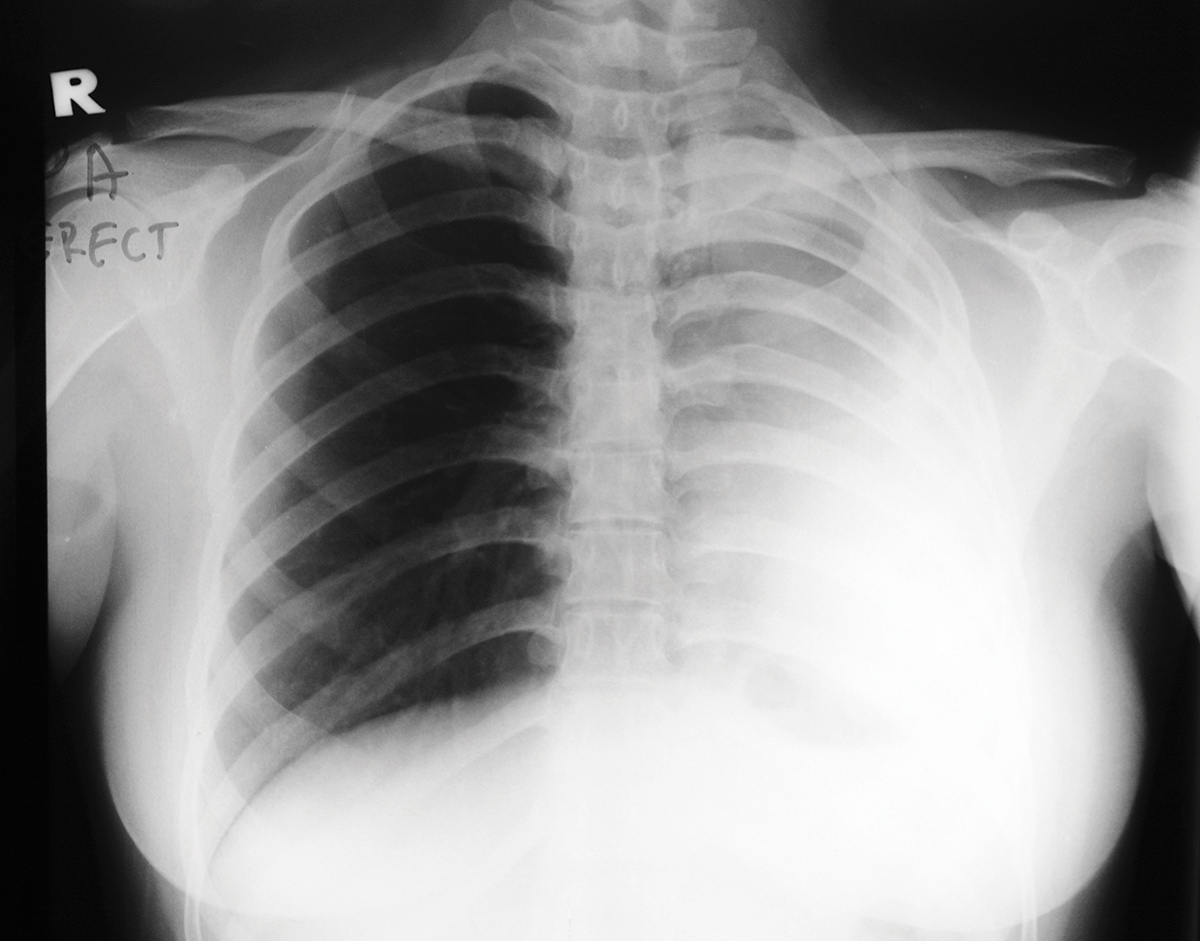
\includegraphics[width=0.6\textwidth,keepaspectratio=true]{lung_opacity}
	\caption{
		RTG z objawami zwłóknienia. Widać małe okrągłe formacje z efektem mlecznej szyby
	}
\end{figure}

%-----------------------------------------------------------------------------------
\subsection{Zapalenie płuc}
Zapaleniem płuc nazywamy stan zapalny przy którym są zapalone pęcherzyki płucne. Przyczyną choroby są zwykle infekcje wirusowe lub bakteryjne. Objawami tej choroby zwykle są gorączka, kaszel, ból w klatce piersiowej, trudność w oddychaniu. Jedną z metod diagnostyki i najbardziej popularną jest metoda robienia zdjęć rentgenowskich. RTG jest narzędziem które pomaga lekarzom diagnozować zapalenie płuc. Na RTG zapalenie widać jako jasny obszar.

\begin{figure}[H]
	\centering
	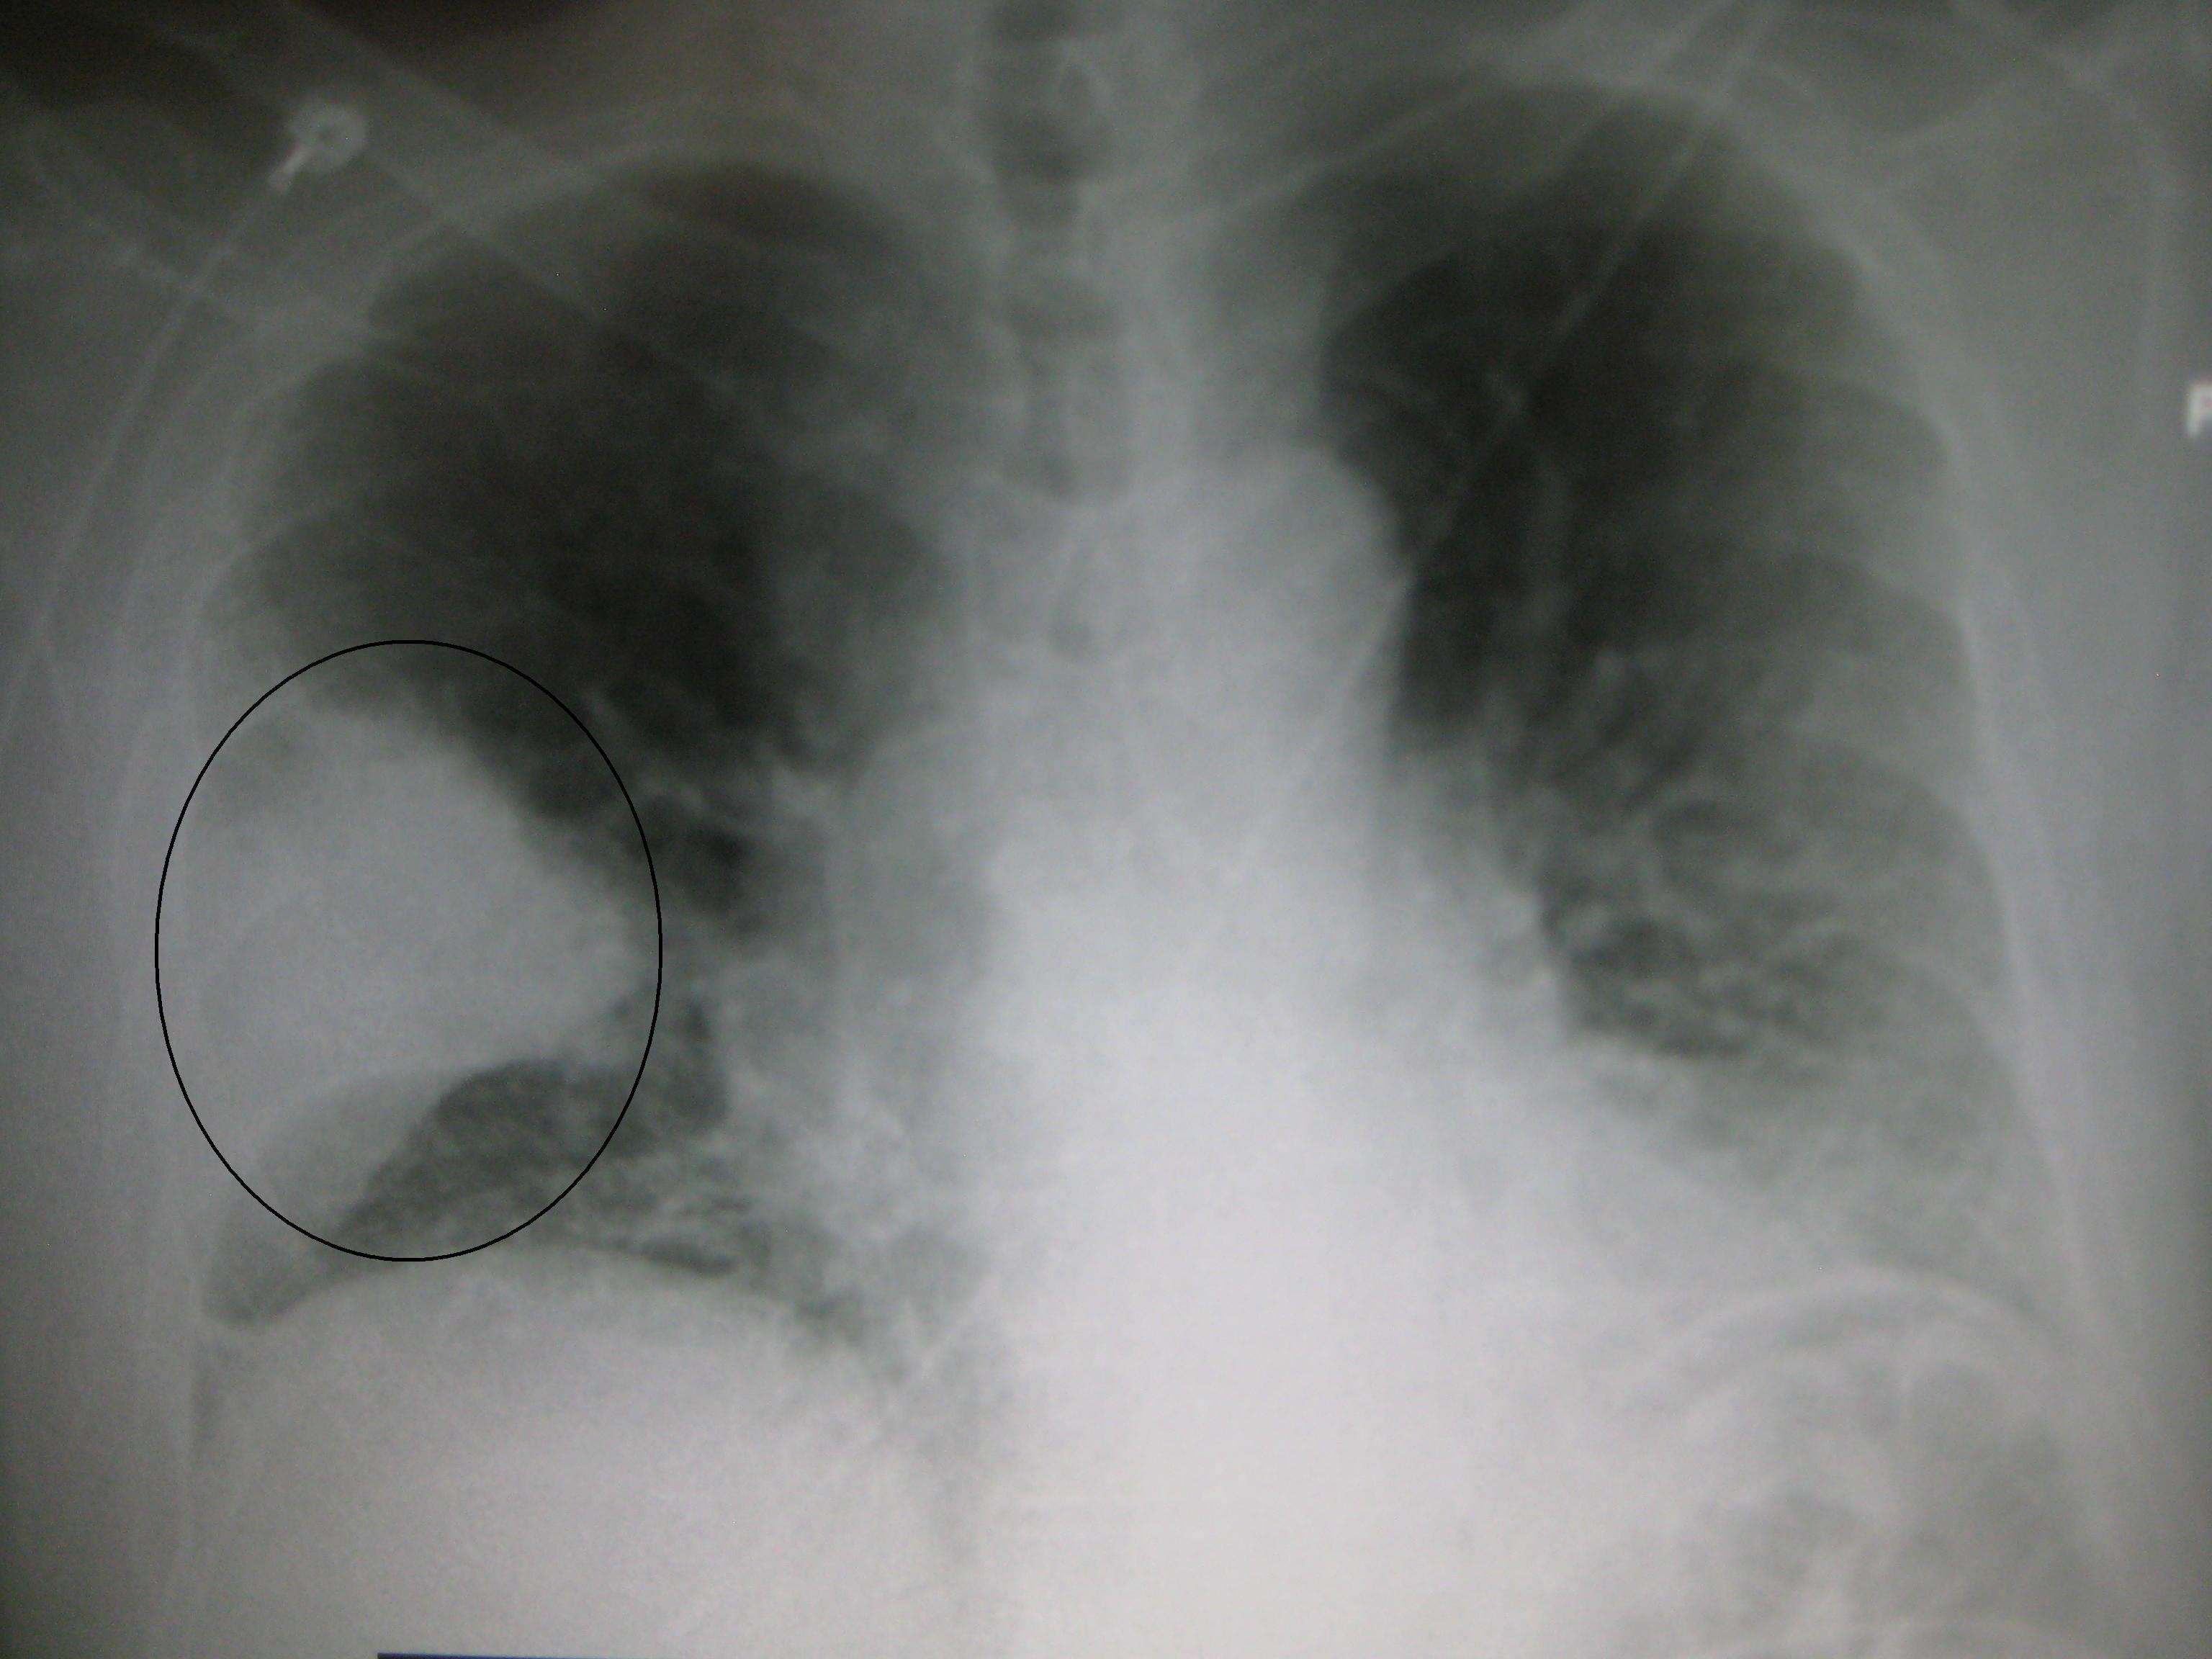
\includegraphics[width=0.6\textwidth,,keepaspectratio=true]{viral_pneumopnia}
	\caption{
		RTG z ostrą formą zapalenia płuc. Obszar z zapaleniem jest jasny i pokazany na rysunku czarnym kołem.
	}
\end{figure}

%-----------------------------------------------------------------------------------
\subsection{COVID-19}
COVID-19 (od ang. \textit{coronavirus disease 2019}) – jest to choroba spowodowana zakażeniem wirusem SARS-CoV-2. Covid może powodować jak efekt mlecznej szyby tak i zapalenie płuc. Metodami diagnozowania są zwykle różnego rodu sprawdzenia krwi na przeciwciała, łańcuchowej reakcji polimerazy oraz komputerowej tomografii. Czasem do diagnozowania przydaje się RTG.

\begin{figure}[H]
	\centering
	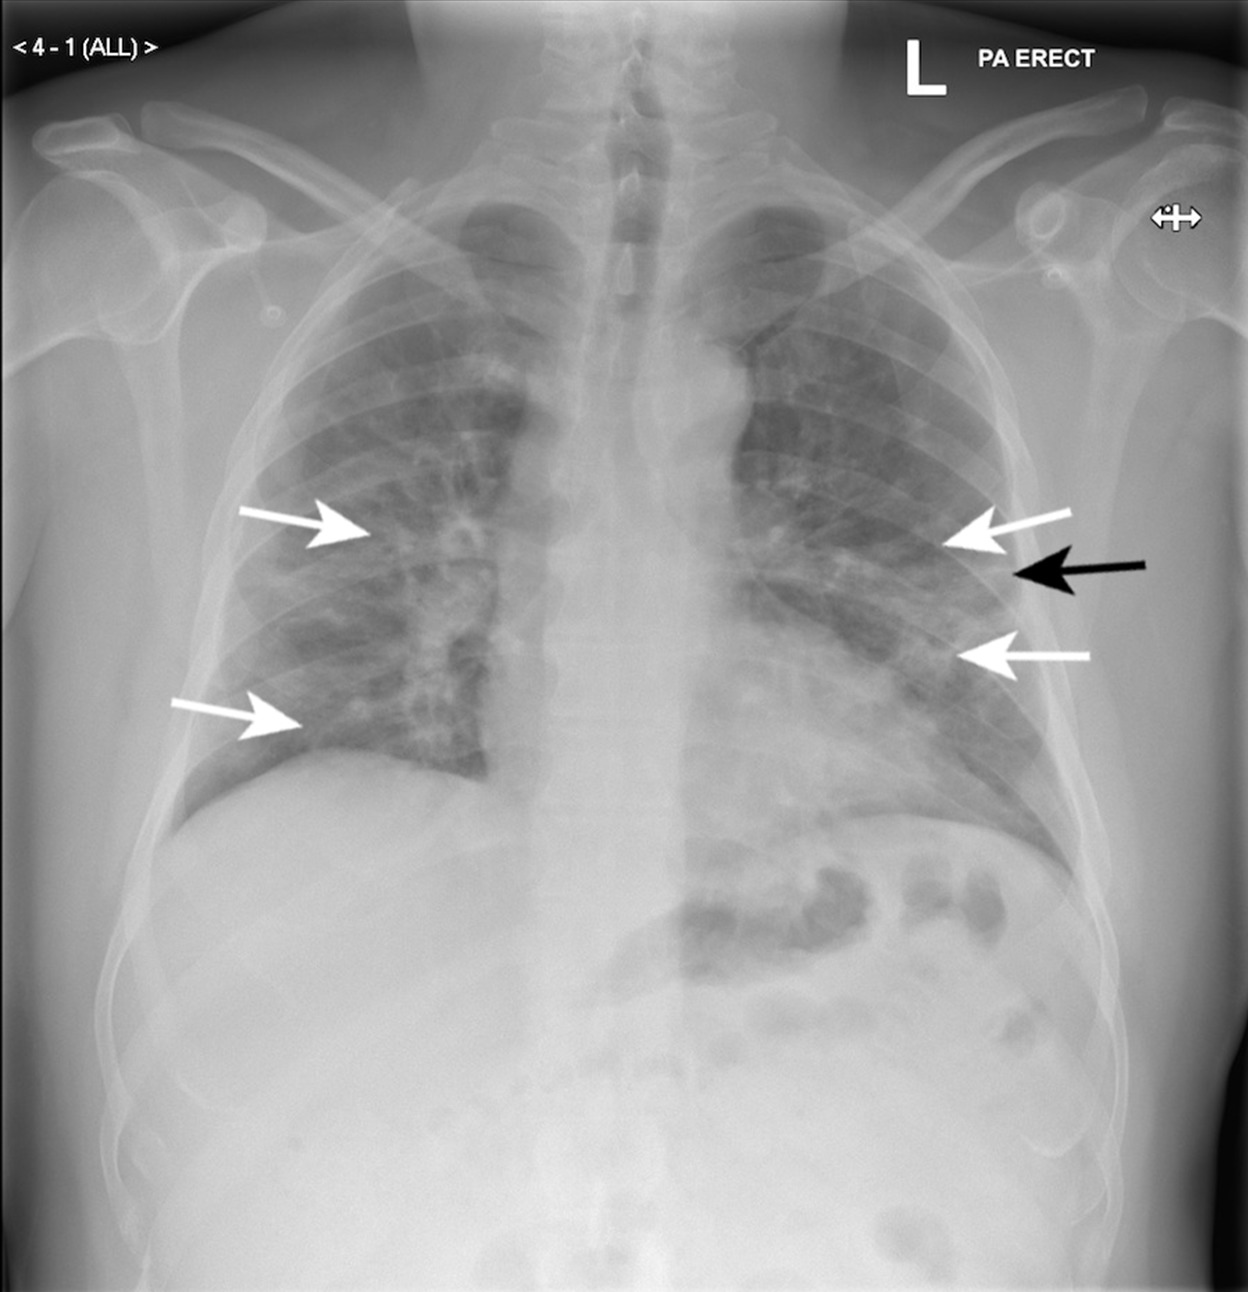
\includegraphics[width=0.6\textwidth,keepaspectratio=true]{covid}
	\caption{
		COVID-19
	}
\end{figure}

%===================================================================================
\section{Uczenie maszynowe}
Uczeniem maszynowym nazywa się dziedzina nauki programowania komputerów w sposób umożliwiający im uczenie się z danych \cite{geron} 
Ta praca jest zrobiona z użyciem uczenia maszynowego a zwłaszcza sieci neuronowych.


%===================================================================================
\section{Neuron}
Zanim opisać sieci neuronowe, będzie przedstawiony neuron (komórka) i z czego się składa.

\subsection{Neuron biologiczny}

Jak wiadomo mózg ludzki i większości innych organizmów składa się z malutkich komórek nerwowych, nazywanych neuron. Neurony przeprowadzają przez siebie sygnał elektryczny. I w ten sposób mogą przetwarzać różną informację Podstawą nerwowego układu zwierząt są Neurony. Mózgowie oraz rdzeń kręgowy stanowią ośrodkowy układ neuronowy który zawiera najwięcej neuronów. \cite{neuroscience}
Jednostka komórkowa (neuron) skłąda się z ciała które zawiera jądro i różne organelli i wypustek: wiele mniejszych dendrytów, jedna długa -- akson. \cite{geron}

\begin{figure}[H]
	\centering
	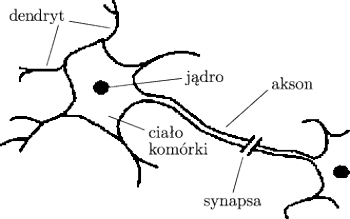
\includegraphics[width=\textwidth,height=6cm,keepaspectratio=true]{neuron_bio}
	\caption{
		Obraz komórki biologicznej \cite{neuron_bio}
	}
\end{figure}

Interakcja między neuronami odbyła się za pomocą impulsów które generują się w ciele komórki i przenoszą się  wzdłuż aksonów. Związek dendryta i aksonu nazywa się synaps. Sygnały to są elektryczne impulsy, które powodują chemiczne reakcji w synapsach. Żeby komórka utworzyła sygnał musi otrzymać dostateczną ilość neuroprzekaźników (uwalnianie w synapsach). Neuroprzekaźniki generują się za pomocą sygnałów elektrycznych przenoszonych wzdłuż aksonów. Ile tych neuroprzekaźników trzeba dla generacji sygnału zależy od samych neuroprzekaźników, niektóre mogą hamować aktywność neuronu.\cite{geron}
Neurony łączą się z dużą ilością innych neuronów, w rezultacie tworzy się wielka sieć. Dla tego że takie proste elementy jak neurony tworzą bardzo wielką i rozgałęzioną sieć, ona może wykonywać różne trudne obliczenia i przetwarzanie danych.\cite{geron}

%-----------------------------------------------------------------------------------
\subsection{Sztuczny neuron}
W 1943 Warren S. McCulloch i Walter Pitts opisali reprezentacje bardzo prostego neuronu sztucznego. Ma on jedno wyjście i wejście w formacie binarnym. Natomiast wejść może być więcej niż jedno ale wyjście tylko jedno. Komórka zostanie aktywna (będzie wysyłała sygnał dalej) jeśli na wejściu będzie określona ilość aktywnych sygnałów.\cite{mcculloch1943logical} Tak prosty model daje nam bardzo duże możliwości. Twórcy udowodnili że za pomocą takich neuronów jesteśmy w stanie zaprotestować sieć która rozwiąże dowolne zadanie logiczne.

Frank Rossenblatt trochę zmodyfikował ten neuron.\newline
Kluczowe zmiany:
\begin{itemize}
	\item Wartościami wejść/wyjść są liczby
	\item Każde połączenie ma przyporządkowaną wagę.
	\item Używanie funkcji skokowej na końcu
	\item Dodatkowe obciążeniowe wejście(zawsze wysyła wartość 1) z własną wagą, tak zwany bias
\end{itemize}

Jednostka wylicza ważoną sumę sygnałów wejściowych, a następnie zostaję użyta funkcja aktywacji. Najczęściej zostaje użyta funkcja skokowa Heaviside`a (Rysunek \ref{Heaviside}) lub signum (Rysunek \ref{Signum}) .Przy użyciu skokowej funkcji aktywacji taki neuron można nazywać progową jednostką logiczną lub liniową jednostką progową (ang. \textit{Linear Treshod Unit} -- LTU). Działanie tej jednostki można matematycznie opisać w następujący sposób.\newline\newline
$ y = \mathcal{H}(W^{T}X + b) $\newline \newline
Gdzie: \newline
X -- wektor wejść. \newline
W -- wektor wag. \newline
b -- bias. \newline
y -- wyjście neuronu. \newline
$ \mathcal{H}(...) $ -- funkcja skokowa Heaviside`a\newline

\begin{figure}[H]
	\centering
	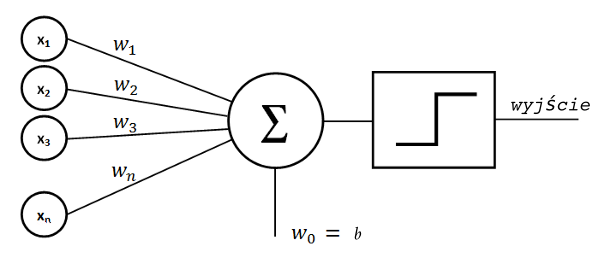
\includegraphics[width=0.8\textwidth,keepaspectratio=true]{neuron_rosenblatta}
	\captionof{figure}{
		Sztuczny neuron Franka Rosenblatta
	}
\end{figure}

%===================================================================================
\section{Funkcji użyte w pracy}

%-----------------------------------------------------------------------------------
\subsection{Funkcja skokowa Heaviside’a}
Funkcja skokowa Heaviside’a, skok jednostkowy – funkcja nieciągła, która przyjmuje wartość dla ujemnych argumentów i wartość 1 w pozostałych przypadkach:

\begin{equation}
	\mathcal{H}(x) = 
	\begin{cases}
		0 & \text{dla $x < 0$}\\
		1 & \text{dla $x \geqslant 0$ }\\
	\end{cases}    
\end{equation}

\begin{figure}[H]
	\centering
	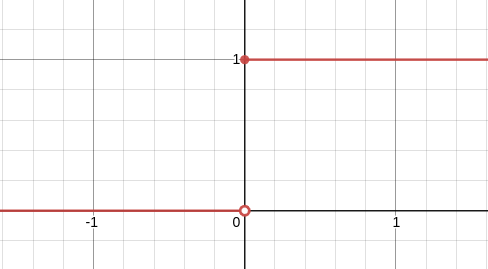
\includegraphics[width=0.6\textwidth,keepaspectratio=true]{Heaviside}
	\caption{
		Funkcja skokowa Heaviside’a
	}
	\label{Heaviside}
\end{figure}


%-----------------------------------------------------------------------------------
\subsection{Signum}
Signum, sgn (łac. signum „znak”) – funkcja zmiennej rzeczywistej, zdefiniowana następująco:
\begin{equation}
	sgn(x) = 
	\begin{cases}
		-1 & \text{dla $x < 0$}\\
		0 & \text{dla $x = 0$}\\
		1 & \text{dla $x > 0$}\\
	\end{cases}    
\end{equation}

\begin{figure}[H]
	\centering
	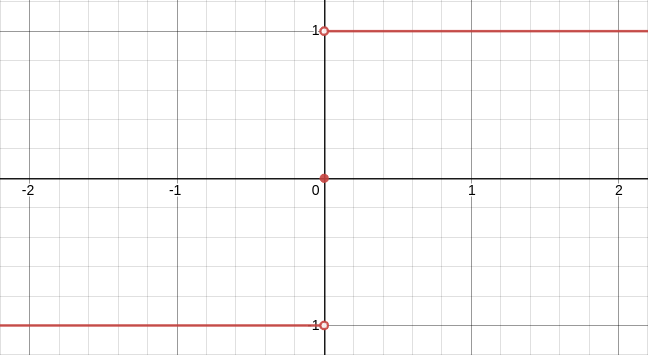
\includegraphics[width=0.6\textwidth,keepaspectratio=true]{Signum}
	\caption{
		Signum
	}
	\label{Signum}
\end{figure}


%-----------------------------------------------------------------------------------
\subsection{Sigmoid}
Kształt funkcji sigmoidalnej jest podobny do litery obróconej litery „S”.
Przykład tej funkcji jest pokazana na rysunku \ref{Sigmoid} i zdefiniowana wzorem: 


\begin{figure}[H]
	\begin{center}
		$S(x) = \dfrac{1}{1 + e^{-x}}$
	\end{center}
	
	\centering
	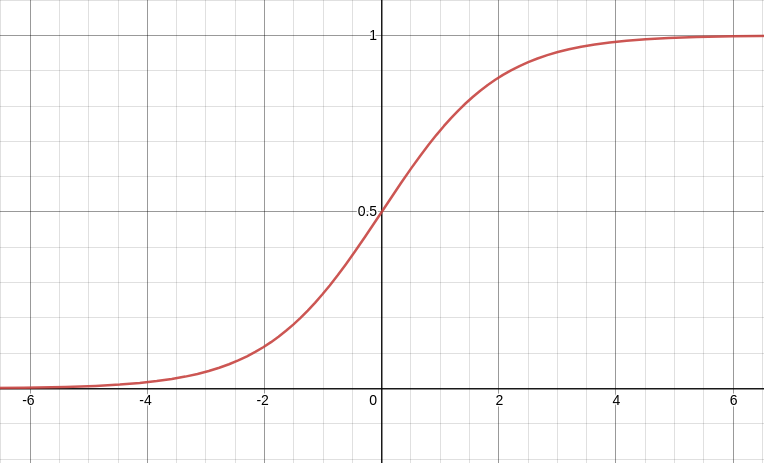
\includegraphics[width=0.6\textwidth,keepaspectratio=true]{Sigmoid}
	\caption{
		Sigmoid
	}
	\label{Sigmoid}
\end{figure}

%-----------------------------------------------------------------------------------
\subsection{ReLU}
Kolejną, popularną funkcją aktywacji jest ReLU (rectifier Linear Unit). Po lewej stronie od osi Y jest równa 0 po prawej -- równomiernie rośnie
\begin{equation}
	ReLU(x) = 
	\begin{cases}
		0 & \text{dla $x < 0$}\\
		x & \text{dla $x \geqslant 0$ }\\
	\end{cases}    
\end{equation}

\begin{figure}[H]
	\centering
	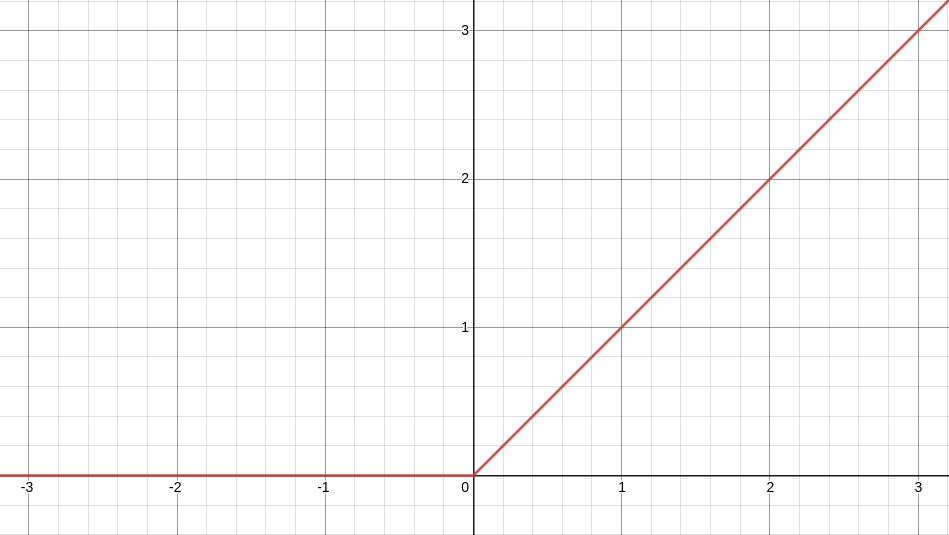
\includegraphics[width=0.6\textwidth,keepaspectratio=true]{ReLu}
	\caption{
		ReLU
	}
\end{figure}

%-----------------------------------------------------------------------------------
\subsection{Softmax}
Funkcja softmax przyjmuje jako dane wejściowe wektor z $K$ liczb rzeczywistych i normalizuje go do rozkładu prawdopodobieństwa składającego się z $K$ prawdopodobieństw proporcjonalnych do wykładników liczb wejściowych. Oznacza to, że przed zastosowaniem softmaxa niektóre składowe wektora mogą być ujemne lub większe niż jeden; i może nie sumować się do 1; ale po zastosowaniu softmaxu każdy składnik będzie w przedziale $[0,1]$, a składniki będą sumować się do 1, aby można je było interpretować jako prawdopodobieństwa. Co więcej, większe komponenty wejściowe będą odpowiadać większym prawdopodobieństwu.

\begin{center}
	\begin{equation}	
		z = Softmax(t) = \mathcal{S}(t) = \dfrac{e^{t_i}}{\sum_{j=1}^{K}e^{t_j}}\text{\quad dla i = ,...,K.}
		\label{softmax}
	\end{equation}
	\ref{softmax}: Obliczanie Softmax
\end{center} 

\begin{flushleft}
	Gdzie:\newline
	K -- ilość neuronów warstwy wyjściowej\newline
	t -- wektor wyjść
	
\end{flushleft}

%-----------------------------------------------------------------------------------
\subsection{Entropia krzyżowa, Cross-Entropy}
Entropia krzyżowa jest funkcją kosztu. Oznacza odległość między dwoma rozkładami prawdopodobieństw.

\begin{center}
	\begin{equation}	
		CE(z, y) = -\sum_{i=1}^{K}y_i \log z_i
		\label{CrossEntropy}
	\end{equation}
	\ref{CrossEntropy}: Obliczanie entropii krzyżowej
\end{center} 

\begin{flushleft}
	Gdzie:\newline
	$z$, $y$ -- rozkłady prawdopodobieństw
\end{flushleft}

%===================================================================================
\section{Sieć neuronowa}
Sieć neuronowa to połączenie neuronów w jakiś sposób. Najbardziej popularne są sieci całkowicie powiązane, jednokierunkowe (ang. \textit{feedforward, fully connected}) albo "dense".

\begin{figure}[H]
	\centering
	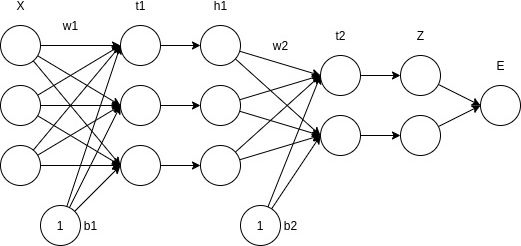
\includegraphics[width=0.6\textwidth,keepaspectratio=true]{feed_forward_network}
	\caption{
		Sieć neuronowa  
	}
	\label{feed_forward_network}
\end{figure}

Na rysunku \ref{feed_forward_network} jest pokazana sieć neuronowa składająca się z trzech warstw: jednej warstwy wejściowej, jednej wyjściowej i jednej ukrytej. Dla ułatwienia obliczeń wektorów wyjść ukrytej i wyjściowej warstwy, obliczania są podzielone na dwie fazy: liniową $X \rightarrow t_1; h_1 \rightarrow t_2$ i nieliniową $t_1 \rightarrow h_1; t_2 \rightarrow z$.

\begin{flushleft}
	$X$ -- wektor wejść (pierwszej warstwy) \newline
	$W_1, W_2$ -- matrycy wag drugiej i trzeciej warstw \newline
	$b_1, b_2$ -- wektory wag biasów drugiej i trzeciej warstw \newline
	$t_1, t_2$ -- liniowe wyjścia drugiej i trzeciej warstw w postaci wektorów\newline
	$h_1$ -- nieliniowe wyjście drugiej warstwy, wektor \newline
	$z$ -- wektor wyjść Softmax \newline
	$E$ -- skalar błędu
\end{flushleft}

\begin{figure}[H]
	\centering
	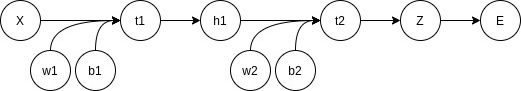
\includegraphics[width=0.6\textwidth,keepaspectratio=true]{feed_forward_graph}
	\caption{
		Graf obliczenia wyjścia sieci i błędu  
	}
	\label{feed_forward_graph}
\end{figure}


Obliczamy wszystko po kolei. Jest sprawą dość prostą. Dla obliczenia wektora wyjścia z każdej warstwy sieci potrzebujemy mieć matrycy wag i wektory biasów. Najcięższej one są inicjalizowane losowo

\begin{flushleft}
Dla obliczenia pierwszej fazy pierwszej warstwy potrzebne są matryca wag i wektor biasów tej warstwy. Wektor wejść tej warstwy mnożymy przez matryce wag i dodajemy wektor biasów.\\
$t_1 = XW_1 + b_1;$\\
\vspace{0.5cm}

Dla obliczenia drugiej fazy(nieliniowej) poprzedni rezultat przeprowadzamy przez funkcje aktywacji.\\
$h_1 = F(t_1);$\\
\vspace{0.5cm}

Metoda obliczania każdej następnej warstwy sieci neuronowej (obliczanie wektorów, czasami matryc lub tensorów. To zależy od wymiarowości danych treningowych) jest dokładnie taka sama. Wektor wejść tej warstwy mnożymy przez matryce wag i dodajemy wektor biasów.\\
$t_2 = h_1W_2 + b_2;$\\
\vspace{0.5cm}

Ostatnia warstwa zwykle ma Softmax jako funkcje aktywacji.\\
$z = \mathcal{S}(t_2);$\\
\vspace{0.5cm}

Dla otrzymania skalaru błędu jest wykorzystana metoda entropii krzyżowej.\\
$E = CE(z,y);$

\end{flushleft}


%===================================================================================
\section{Nadzorowane uczenie sztucznych sieci neuronowych}
Proces uczenia sieci polega na tym że zmieniamy wagi neuronów i biasów w sposób który prowadzi do zmniejszenia błędu na wyjściu sieci. Zmierzyć ten błąd nie jest trudno, wyżej to już zostało opisane. Uczenie składa się z dwóch etapów: etapu obliczenia gradientu i etapu optymizacji wag. 
Dla pierwszego etapu w swojej prace używam algorytmu propagacji wstecznej (ang. \textit{back propagation}). Natomiast dla etapu optymizacji używam optymizatora Adaptive Moment Estimation (Adam)

%===================================================================================
\section{Propagacja wsteczna}
Najbardziej popularnym algorytmem uczenia nadzorowanego jest propagacja wsteczna jak mówi jej nazwa ona przeprowadza coś wstecz, czyli od końca na początek. Tak naprawdę on jest stosowany tylko wielowarstwowych jednokierunkowych sieci neuronowych. To co on robi to przeprowadza błąd uczenia od wyjścia do wejścia, a dokładniej pochodną błędu, która pomaga zrozumieć w która stronę trzeba zmieniać parametry sieci żeby zmniejszyć błąd. \cite{nn_jozef}

%-----------------------------------------------------------------------------------
\subsection{Znależenie gradientu ostatniej warstwy}
\begin{figure}[H]
	\centering
	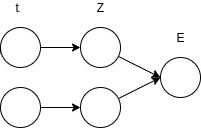
\includegraphics[width=0.3\textwidth,keepaspectratio=true]{feed_forward_error}
	\caption{Osobno narysowana ostatnia warstwa sieci na rysunku \ref{feed_forward_network}}
	\label{feed_forward_error}
\end{figure}

\begin{flushleft}
Wyliczanie wyjścia Softmax\\
$z = Softamx(t) = \mathcal{S}(t)= \frac{e^{t_i}}{\sum_{j=1}e^{t_i}}$ \\
\vspace{0.5cm}

Do wyliczania skalaru błędu potrzebujemy $z$ - wektor wyjść sieci oraz $y$ - wektor poprawnej odpowiedzi w postaci wektora z taką samą wymiarowością jak i wektor wyjścia sieci.\\
$E = CrossEntropy(z, y) = -\sum_{i=1}y_i\log z_i$\\
\vspace{0.5cm}

W tym przypadku błąd jest wyliczany w ten sposób, z użyciem formuły Softmax\\
$E = CE(\mathcal{S}(t),y)=-\sum_{i=1}y_i\log\frac{e^{t_i}}{\sum_{j=1}e^{t_i}}$\\
$= -\sum_{i=1}y_i(t_i-\log \sum_{j=1}e^{t_i}) =$\\
$= -\sum_{i=1}y_it_i + \sum_{i=1}y_i\log\sum_{j=1}e^{t_i} =$\\
$= -\sum_{i=1}y_it_i + \log\sum_{j=1}e^{t_i}$\\
Po nietrudnych przekształceniach otrzymujemy powyższą formułę.\\
\vspace{0.5cm}

Do propagacji wstecznej jest potrzebna pochodna błędu. Można bardzo łatwo ją policzyć dla poszczególnego neuronu $t_k$ -- k-ty neuron warstwy $t$ \\
$\frac{\delta E}{\delta t_k} = -y_k + \frac{1}{\sum_{j=1}e^{t_j}}\cdot e^{t_k} = \mathcal{S}_k - y_k$\\
\vspace{0.5cm}

Można zauważyć że otrzymaliśmy wzór na Softmax. Czyli pochodną błędu po wyjściu warstwy t można bardzo łatwo policzyć, po prostu, od wektora wyjść sieci odjąć wektor oczekiwany.\\ 
$\frac{\delta E}{\delta t} = \mathcal{S}(t) - y = z - y$
\end{flushleft}

\begin{figure}[H]
	\centering
	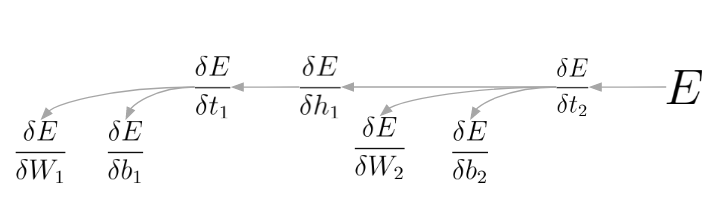
\includegraphics[width=0.6\textwidth,keepaspectratio=true]{gradient_graph}
	\caption{Graf obliczenia gradientu}
	\label{gradien_graph}
\end{figure}

\begin{flushleft}
Obrachunki otrzymania reszty pochodnych:\\
$\dfrac{\delta E}{\delta t_2} = S(t_2)-y=z-y$\\
\vspace{5mm}
$\dfrac{\delta E}{\delta W_2} = h_1^T \cdot \dfrac{\delta E}{\delta t_2}$\\
$\dfrac{\delta E}{\delta b_2} = \dfrac{\delta E}{\delta t_2}$\\
\vspace{5mm}
$\dfrac{\delta E}{\delta h_1} = \dfrac{\delta E}{\delta t_2} \cdot W_2^T$\\
$\dfrac{\delta E}{\delta t_1} = \dfrac{\delta E}{\delta h_1} \odot F^\prime (t_1)$\\
\vspace{5mm}
$\dfrac{\delta E}{\delta W_1} = X^T \cdot \dfrac{\delta E}{\delta t_1}$\\
$\dfrac{\delta E}{\delta b_1} = \dfrac{\delta E}{\delta t_1}$
\end{flushleft}

%===================================================================================
\section{Splotowe sieci neuronowe}
Jak wiadomo do wizji komputerowej już od dawna używają sieci neuronowe. Ale jeśli używać do tego zwykłych neuronów powiązanych w sieci feedforward, fully connected, to będziemy mieli za dużo wag. Przypuśćmy że mamy kolorowy obrazek 200x200 pikseli. Ilość neuronów będzie 200*200*3=120000. Już mamy bardzo dużo neuronów przecież to tylko warstwa wejściowa. Jeżeli następna warstwa będzie miała 512 neuronów (co jest rzeczywiście za mało), to w pierwszej warstwie będzie 61440000 wag. Jest to bardzo dużo. 
Splotowe sieci, wymyślone w latach 80 ubiegłego wieku, mogą ulepszyć sytuacje.

%-----------------------------------------------------------------------------------
\subsection{Struktura kory wzrokowej}
Dzięki eksperymentom David H. Hubel nieprzeprowadzonych na kotach wiemy jak działa kora wzrokowa.\cite{David_1958} \cite{David_1959}
Udowodnili one że każdy neuron odpowiada za swoje pole recepcyjne czyli określony rejon pola wzrokowego. I reagują tylko na obiekty, mieszczące się ich polu (Rysunek \ref{kora_wzrokowa}). \cite{geron}

Również było pokazane że neurony mimo tego że reagują na określone pole, jeszcze reagują na pewny kształt. Mogą to być zarówno linie powożone pod różnym kątem tak i inne figury. Pola recepcyjne mogą różnić się rozmiarem i skomplikowaniem kształtu na który reagują. Neurony, które są połączone z neuronami co reagują na proste kształty mogą wykrywać coś bardziej skomplikowanego. Tworzą one tak zwane warstwy gdzie każdy neuron poszczególnej warstwy jest połączony z kilkoma komórkami poprzedniej warstwy (rysunek \ref{kora_wzrokowa}). Taka architektura pozwala wykrywać wszelkie obiekty i kształty. \cite{geron}

\begin{figure}[H]
	\centering
	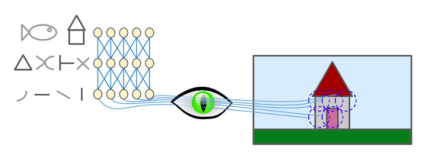
\includegraphics[width=0.6\textwidth,keepaspectratio=true]{kora_wzrokowa}
	\caption{Działanie kory wzrokowej \cite{geron}}
	\label{kora_wzrokowa}
\end{figure}

%-----------------------------------------------------------------------------------
\subsection{Warstwy splotowe}
Podstawą sieci splotowej (ang. \textit{Convolutional Neural Networt, CNN}) jest warstwa splotowa. Gdzie neurony tworzą taką samą architekturę jaka jest w prawdziwej biologicznej korze wzrokowej. Czyli wejście jest dwuwymiarowe, pierwsza warstwa jest połączona z wejściem w ten sposób że każdy neuron jest połączony ze swoim polem recepcyjnym. Z kolei każdy neuron w drugiej warstwie splotowej łączy się wyłącznie z neuronami znajdującymi się w niewielkim obszarze pierwszej warstwy.(rysunek \ref{warstwa_splotowa}).
Przy takiej architekturze sieć rozpoznaje proste kształty w pierwszej warstwie i im głębiej wchodzimy tym bardziej skomplikowane kształty, formy, obiekty zostają sklasyfikowane. \cite{geron}

\begin{figure}[H]
	\centering
	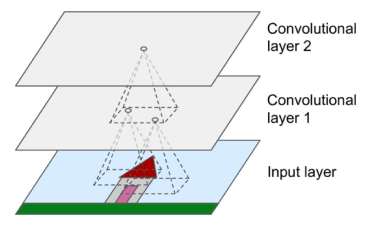
\includegraphics[width=0.6\textwidth,keepaspectratio=true]{warstwa_splotowa}
	\caption{Warstwy CNN \cite{geron}}
	\label{warstwa_splotowa}
\end{figure}

\subsection{Uzupełnianie zerami}
Przypuśćmy że każdy neuron ma pole $3 \times 3$ i pola neuronów nakładają się z krokiem w 1 piksel. To na wyjściu drugie warstwy będziemy mieli obraz rozmiaru o 1 piksel z każdej strony mniejszy od wejściowego obrazu. Żeby rozwiązać ten problem możemy rozszerzyć wejściowy obraz tak samo o jeden piksel z każdej strony. Żeby to zrobić możemy dopisać zera na brzegach obrazu. Ten proces nazywa się uzupełnianie zerami.
\begin{figure}[H]
	\centering
	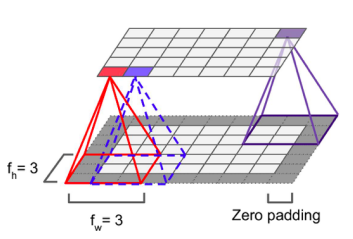
\includegraphics[width=0.6\textwidth,keepaspectratio=true]{padding}
	\caption{Związek pomiędzy warstwami a uzupełnianiem zerami \cite{geron}}
	\label{padding}
\end{figure}

%-----------------------------------------------------------------------------------
\subsection{Krok}
%PLAGIAT
Możliwe jest również łączenie bardzo dużej warstwy wejściowej ze znacznie mniejszą kolejną warstwą poprzez rozdzielanie pól recepcyjnych, tak jak zaprezentowano na rysunku \ref{step}. Rozwiązanie to zmniejsza drastycznie złożoność obliczeniową modelu. Odległość pomiędzy dwoma kolejnymi polami recepcyjnymi nosi nazwę kroku (ang. \textit{stride}). Na widocznym schemacie warstwa wejściowa o wymiarach $5 \times 7$ (plus uzupełnianie zerami) łączy się z warstwą o rozmiarze $3 \times 4$ za pomocą pól recepcyjnych będących kwadratami $3 \times 3$ i kroku o wartości 2 (w omawianym przykładzie krok jest taki sam w obydwu wymiarach, ale nie jest to wcale regułą). Neuron zlokalizowany w rzędzie $i$ oraz kolumnie $j$ górnej warstwy łączy się z wyjściami neuronów dolnej warstwy mieszczącymi się w rzędach od $i\times s_{h}$, do $i \times s_{h}+f_{h}-1$ iw kolumnach od $j \times s_{w}$, do $j \times s_{w}+f_{w}-1$. gdzie $s_{h}$ i $s_{w}$, definiują wartości kroków odpowiednio w kolumnach i rzędach. \cite{geron}
\begin{figure}[H]
	\centering
	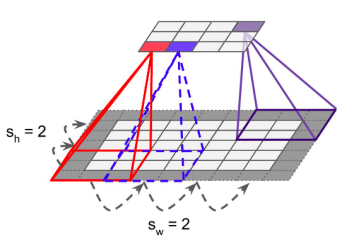
\includegraphics[width=0.6\textwidth,keepaspectratio=true]{step}
	\caption{Redukcja wymiarowości za pomocą kroku o wartość 2 \cite{geron}}
	\label{step}
\end{figure}


%-----------------------------------------------------------------------------------
\subsection{Filtry}
Filtry to są wagi neuronów w warstwach splotowych, mają postać obrazu wielkości pola recepcyjnego. Filtry pomagają wykrywać rożne kształty. Na rysunku \ref{filters} widzimy dwa przykłady filtrów: po lewej stronie mamy filtr, który ma białą pionową linie (jest narysowany obok strzałki). Po prawej stronie, natomiast, jest filtr z poziomą linią. Możemy sobie wyobrazić że przy stosowaniu filtru on jest nakładany na obraz w polu recepcyjnym wybranego neuronu, piksele które są pod białym kolorem dodają się do sumy tego neuronu, natomiast piksele, które podpadają pod czarny obszar filtru, nie mają żadnego znaczenia. 

Jeśli wszystkie neurony w warstwie będą stosować filtr z pionową linią to uzyskamy obrazek po lewej stronie. Widać że wszystkie pionowe kształty zostają bardziej widoczne, wszystko inne zostaje rozmazane. Natomiast w prawym obrazku jest stosowany poziomy filtr, który wyróżnia tylko poziome kształty.

Obraz który jest generowany za pomocą filtru splotowego nazywa się mapą cech.

\begin{figure}[H]
	\centering
	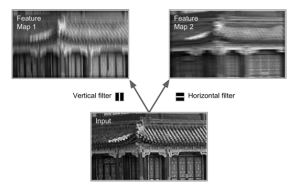
\includegraphics[width=0.8\textwidth,keepaspectratio=true]{filters}
	\caption{Uzyskiwanie map cech za pomocą filtrów \cite{geron}}
	\label{filters}
\end{figure}

%-----------------------------------------------------------------------------------
\subsection{Stosy map cech}
W rzeczywistości warstwy splotowe mają więcej niż dwa wymiary. Najczęstszej są one trójwymiarowe, są to stosy map cech o jednakowym wymiarze. Pole recepcyjne neuronu nie ulega zmianie, ale przebiega przez wszystkie mapy cech poprzednich warstw. Krótko mówiąc, warstwa splotowa równocześnie stosuje różne filtry na wejściach, dzięki czemu jest w stanie wykrywać wiele cech w dowolnym obszarze obrazu \cite{geron}

Stosowanie jednakowych filtrów dla neuronów w jednej warstwie pozwala na znalezienie kształtu w różnych miejscach na zdjęciu. Na przykład, jak filtr będzie szukał litery "A" na zdjęciu to dla sieci splotowej nie ma znaczenia gzie ta litera jest rozmieszczona, natomiast normalna sieć z "fullyconected" warstwami jest w stanie odnaleźć tą literę tylko w jednym miejscu. I stosowanie filtru dla całej warstwy zmniejsza liczbę parametrów, dla tego że nie musimy pamiętać wagi każdego neuronu a tylko filtr, który ma znacznie mniej parametrów od ilości neuronów warstwie\cite{geron}

Co więcej, obrazy wejściowe także mogą być wielowymiarowe, na przykład kolorowy obraz który ma trzy wymiary szerokość, wysokość, i kolor.Kolorowe zdjęcie ma standardowo trzy kanały (czerwony, zielony, niebieski) Czarno-białe obrazy mają tylko jeden kanał odcień szarości, ale istnieją zdjęcia, które mają więcej kanałów jak na przykład fotografie satelitarne utrwalające dodatkowe częstotliwości fal elektromagnetycznych . \cite{geron}

%PLAGIAT
W szczególności neuron zlokalizowany w rzędzie $i$ oraz kolumnie $j$ mapy cech $k$ w danej warstwie splotowej $l$ jest połączony z neuronami wcześniejszej warstwy $l-1$ umieszczonymi w rzędach od $i \times s_{h}$ do $i \times s_{h}+f_{h}-1$ i kolumnach od $j \times s_{w}$, do $j \times s+f_{w}-1$ we wszystkich mapach cech (warstwy $l-1$). Zwróć uwagę, że wszystkie neurony znajdujące się w tym samym rzędzie $i$ oraz kolumnie $j$, ale w innych mapach cech są połączone z wyjściami dokładnie tych samych neuronów poprzedniej warstwy. \cite{geron}

Podsumowanie tego opisu jest w równaniu \ref{conv_formula}
\vspace{1cm}

\begin{center}
	\begin{equation}	
		z_{i,j,k}=b_{k}
		\sum_{u=0}^{f_{h}-1}\sum_{v=0}^{f_{w}-1}\sum_{k^\prime=0}^{f_{n^\prime}-1}
		x_{i^\prime,j^\prime,k^\prime}\cdot w_{u,v,k^\prime,k}
		\quad gdzie \left\{ \begin{array}{ll}
			i^\prime = i \times s_{h}+u\\
			j^\prime = j\times s_{w}+v
		\end{array} \right.
		\label{conv_formula}
	\end{equation}
	\ref{conv_formula}: Obliczanie wartości wyjściowej neuronu w warstwie splotowej
\end{center}

\begin{itemize}
	\item $z_{i,j,k}$ -- wyjście neuronu w $k$ mapie cech w rzędzie $i$ i kolumnie $j$
	\item $f_{h}-1$ i $f_{w}-1$ -- są wysokością i szerokością pola recepcyjnego
	\item $f_{n^\prime}-1$ -- liczba map cech poprzedniej warstwy
	\item $x_{i^\prime,j^\prime,k^\prime}\cdot$ -- wyjście neurony w $k^\prime$ mapie cech w rzędzie $i^\prime$ i kolumnie $j^\prime$ poprzedniej warstwy
	\item $b_{k}$ -- bias dla mapy cech $k$ w tej warstwie
	\item $s_{h}$ i $s_{w}$ -- są kroki: horyzontalny i wertykalny.
	\item $w_{u,v,k^\prime,k}$ -- waga dla każdego neurona w mapie cech $k$ a neuronem w rzędzie $u$, kolumnie $v$ (względem pola recepcyjnego), mapie cech $k^\prime$ 
\end{itemize}

\begin{figure}[H]
	\centering
	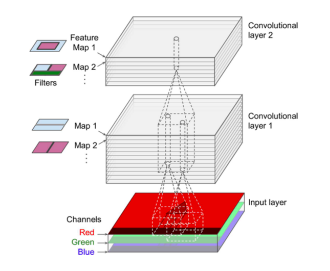
\includegraphics[width=0.6\textwidth,keepaspectratio=true]{stosy_map_cech}
	\caption{Warstwy splotowe zawierające wiele map cech, zdjęcie z trema kanałami barw \cite{geron}}
	\label{stosy_map_cech}
\end{figure}

%-----------------------------------------------------------------------------------
\subsection{Warstwa łącząca (Max pooling)}
Mechanizm działania tej warstwy jest podobny do działania filtrów splotowych. Każda jednostka tej warstwy ma wcześniej określone pole. Różnicą jest w tym że pola nie są nakładane na pola innych neuronów, są rozmieszczone jedno po drugim (można zobaczyć na rysunku \ref{max_pooling}). Wyjściem każdej jednostki będzie maksymalna wartość z pośród wartości na wejściu.

Na przykład w lewym dolnym polu recepcyjnym na rysunku \ref{max_pooling} widzimy wartości wejściowe 1, 5, 3, 2, zatem tylko wartość maksymalna (5) zostanie przekazana do następnej warstwy. \cite{geron}

\begin{figure}[H]
	\centering
	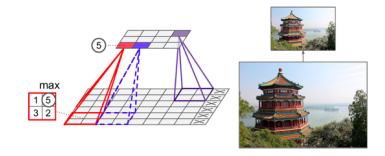
\includegraphics[width=0.8\textwidth,keepaspectratio=true]{max_pooling}
	\caption{Maksymalizująca warstwa łącząca \cite{geron}}
	\label{max_pooling}
\end{figure}


%-----------------------------------------------------------------------------------
\subsection{Warstwa porzucenia (Dropout)}
Ta warstwa stosuje się do zabezpieczenia "dobrego" uczenia, bez przetrenowania. Działa ona w ten sposób że losowo "usuwa",  połączenia między niektórymi neuronami. Jest to bardzo efektywne zabezpieczenie przed przetrenowaniem. Przy inicjalizacji tej warstwy określamy jaki procent połączeń będą "usuwane". Ważną rzeczą jest to że warstwę porzucenia stosujemy tylko w czasie uczenia. Po uczeniu ta warstwa jest usuwana. Czyli sieć działa normalnie, bez wyłączania połączeń. \cite{jak_dziawaja_cnn}


%-----------------------------------------------------------------------------------
\subsection{Warstwa spłaszczająca (Flatten)}
Jest to bardzo prosty i ważny krok. Taka warstwa przetwarza wielowymiarowe wejście w jednowymiarowy wektor. Stosuje się tego żeby połączyć warstwę splotową i w pewni połączoną. Na przykład tensor o wielkości (10, 10, 3) zostałby przekształcony w wektor o rozmiarze 300 (1, 300). \cite{jak_dziawaja_cnn}

%===================================================================================
\section{Implementacja}
Dla klasyfikacji chorób płuc a głownie COVID-19 zdecydowałem na wykorzystanie splotowej sieci z następnym przejściem w zwykłą sieć jednokierunkową, całkowicie powiązaną. Co w teorii w warstwach splotowych daje możliwość sieci najpierw zauważyć różne kształty, cechy a następnie za pomocą zwykłej sieci neuronowej poprawnie zaklasyfikować chorobę.

%-----------------------------------------------------------------------------------
\subsection{Ostateczna struktura sieci}
Po kilku próbach i eksperymentach ostateczną strukturą sieci jest pięć warstw splotowych które są rozmieszczone na przemian z warstwami łączącymi, na końcu są trzy warstwy zwykłych. Wszystkie warstwy oprócz ostatniej mają funkcje aktywacji ReLU, ostatnia warstwa korzysta z Softmax. Sieć zawiera 16,983,268 parametrów.\\

A dokładniej:
\begin{itemize}
	\item Warstwa wejściowa z wymiarami (299,299,1)
	
	\item Warstwa splotowa. 32 filtry o rozmiarach (5,5)
	\item Warstwa łącząca o rozmiarze (2,2)
	\item Dropout 25\%
	
	\item Warstwa splotowa. 32 filtry o rozmiarach (3,3)
	\item Warstwa łącząca o rozmiarze (2,2)
	\item Dropout 25\%
	
	\item Warstwa splotowa. 64 filtry o rozmiarach (3,3)
	\item Warstwa łącząca o rozmiarze (2,2)
	\item Dropout 25\%
	
	\item Warstwa splotowa. 64 filtry o rozmiarach (3,3)
	\item Warstwa łącząca o rozmiarze (2,2)
	\item Dropout 25\%
	
	\item Warstwa splotowa. 128 filtry o rozmiarach (3,3)
	\item Warstwa łącząca o rozmiarze (2,2)
	\item Dropout 25\%
	
	\item Warstwa spłaszczająca
	\item Dropout 25\%
	
	\item W pełni powiązana warstwa zawierająca 512 neuronów
	\item Dropout 50\%
	
	\item W pełni powiązana warstwa zawierająca 128 neuronów
	\item Dropout 50\%
	
	\item Warstwa wyjściowa zawierająca 4 neurony
\end{itemize}


%-----------------------------------------------------------------------------------
\subsection{Historia uczenia}
\begin{figure}[H]
	\centering
	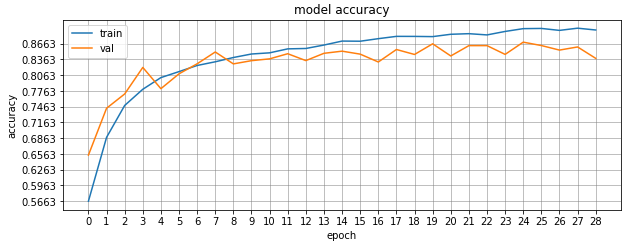
\includegraphics[width=1\textwidth,keepaspectratio=true]{accuracy}
	\caption{}
	\label{accuracy}
\end{figure}

\begin{figure}[H]
	\centering
	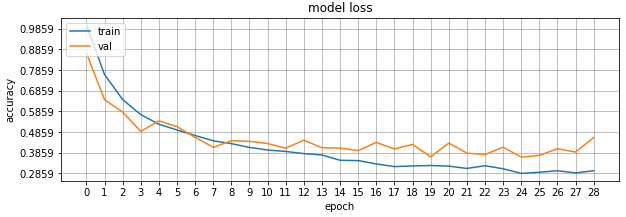
\includegraphics[width=1\textwidth,keepaspectratio=true]{loss}
	\caption{}
	\label{loss}
\end{figure}

Patrząc na wykres historii możemy zobaczyć że przetrenowania wielkiego niema. na końcu rezultat dla danych treningowych jest troszeczkę lepszy co jest całkiem normalną sytuacją. Trochę jest dziwne to że na samym początku dane testowe dają lepszy rezultat, to może nam mówić o tym że mamy nie zbyt dobre dane treningowe i testowe. Najlepszy rezultat był osiągnięty w 24 powtórzeniu. Żeby nie stracić właściwie wytrenowane wagi, po każdej iteracji był robiony backup wag które dają najlepszy rezultat. 
%-----------------------------------------------------------------------------------
\subsection{Stosy map cech}

Żeby lepiej zrozumieć co się dzieje w środku sieci został napisany skrypt który wyświetla mapy cech dla każdej warstwy splotowej.

\begin{figure}[H]
	\centering
	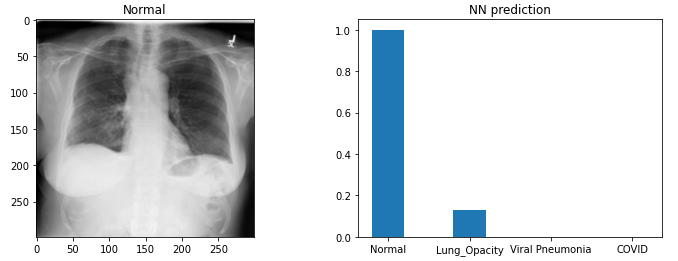
\includegraphics[width=1\textwidth,keepaspectratio=true]{normal_prediction}
	\caption{Predykcja losowego zdjęcia zdrowych płuc ze zbioru testowego.}
	\label{normal_pediction}
\end{figure}

\begin{figure}[H]
\centering
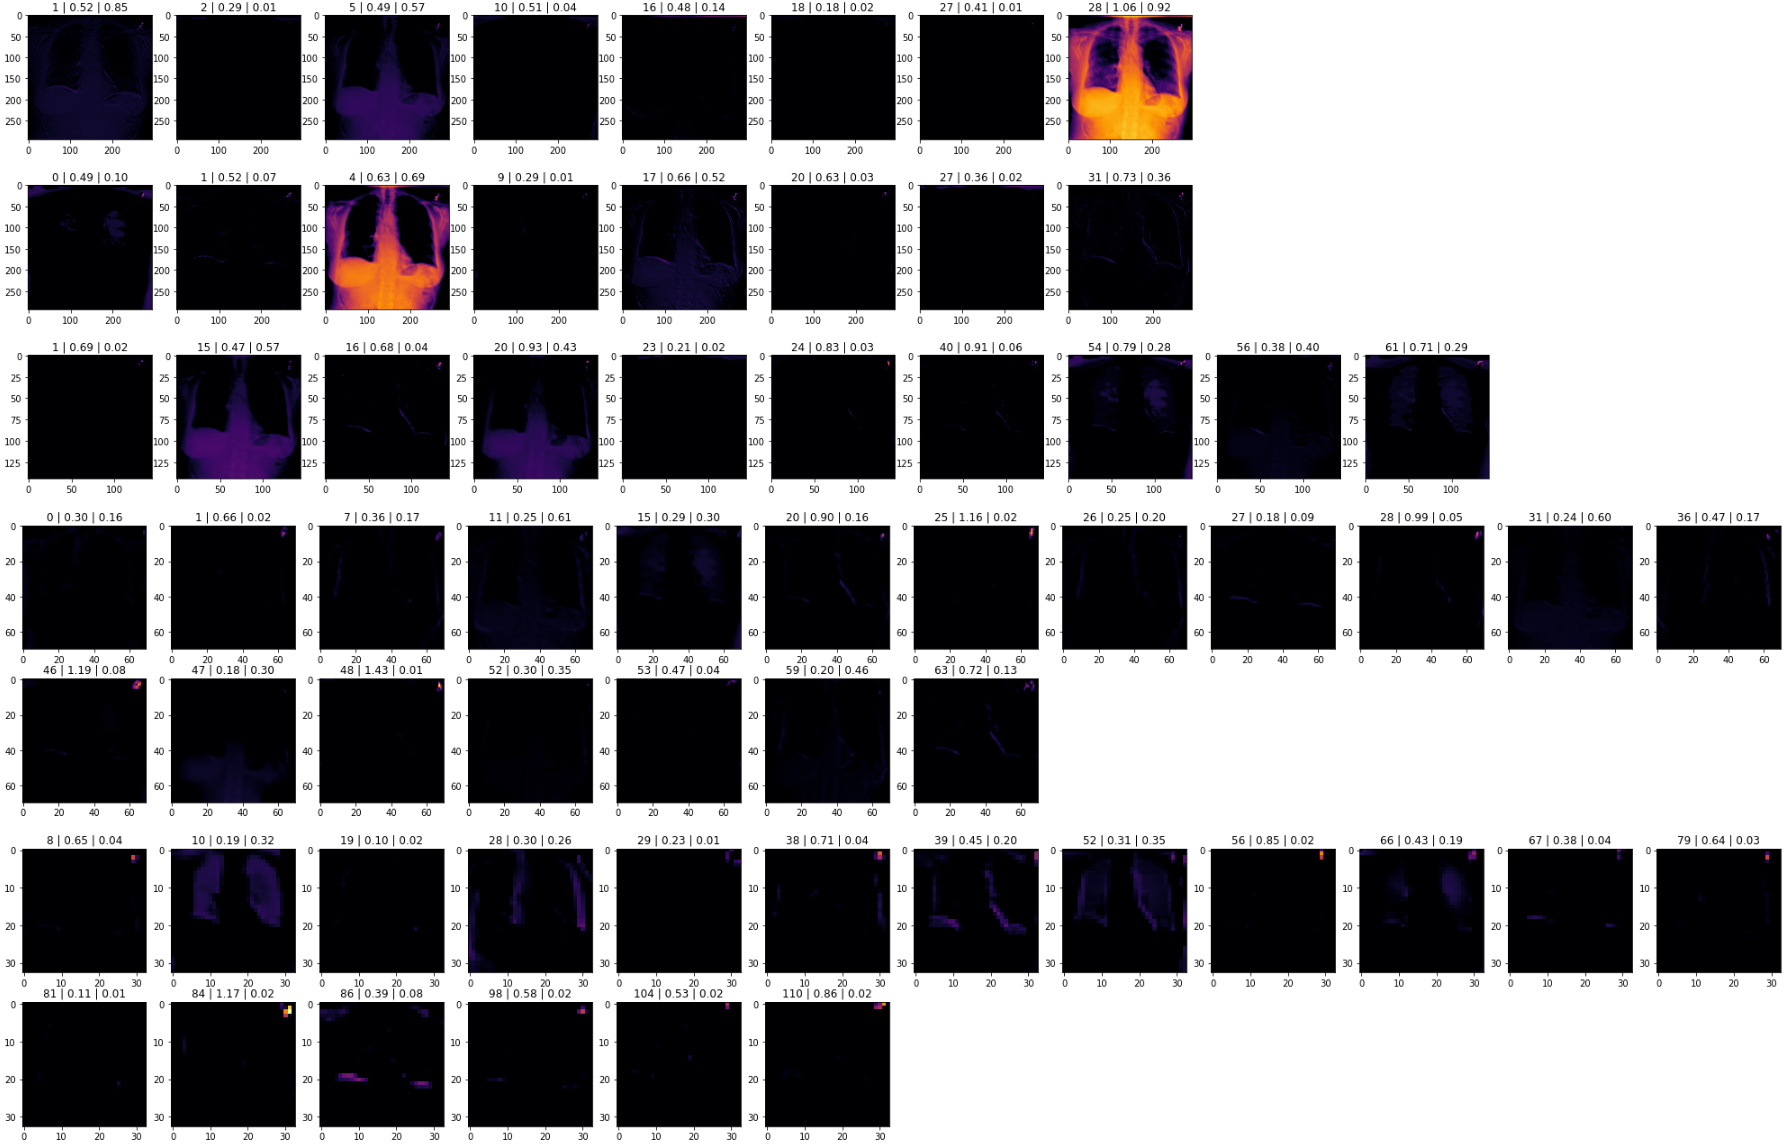
\includegraphics[width=1\textwidth,keepaspectratio=true]{normal_filters_dark}
\caption{Mapy cech generowane pod czas predykcji obrazu na poprzednim rysunku}
\label{normal_filters_dark}
\end{figure}

\begin{figure}[H]
\centering
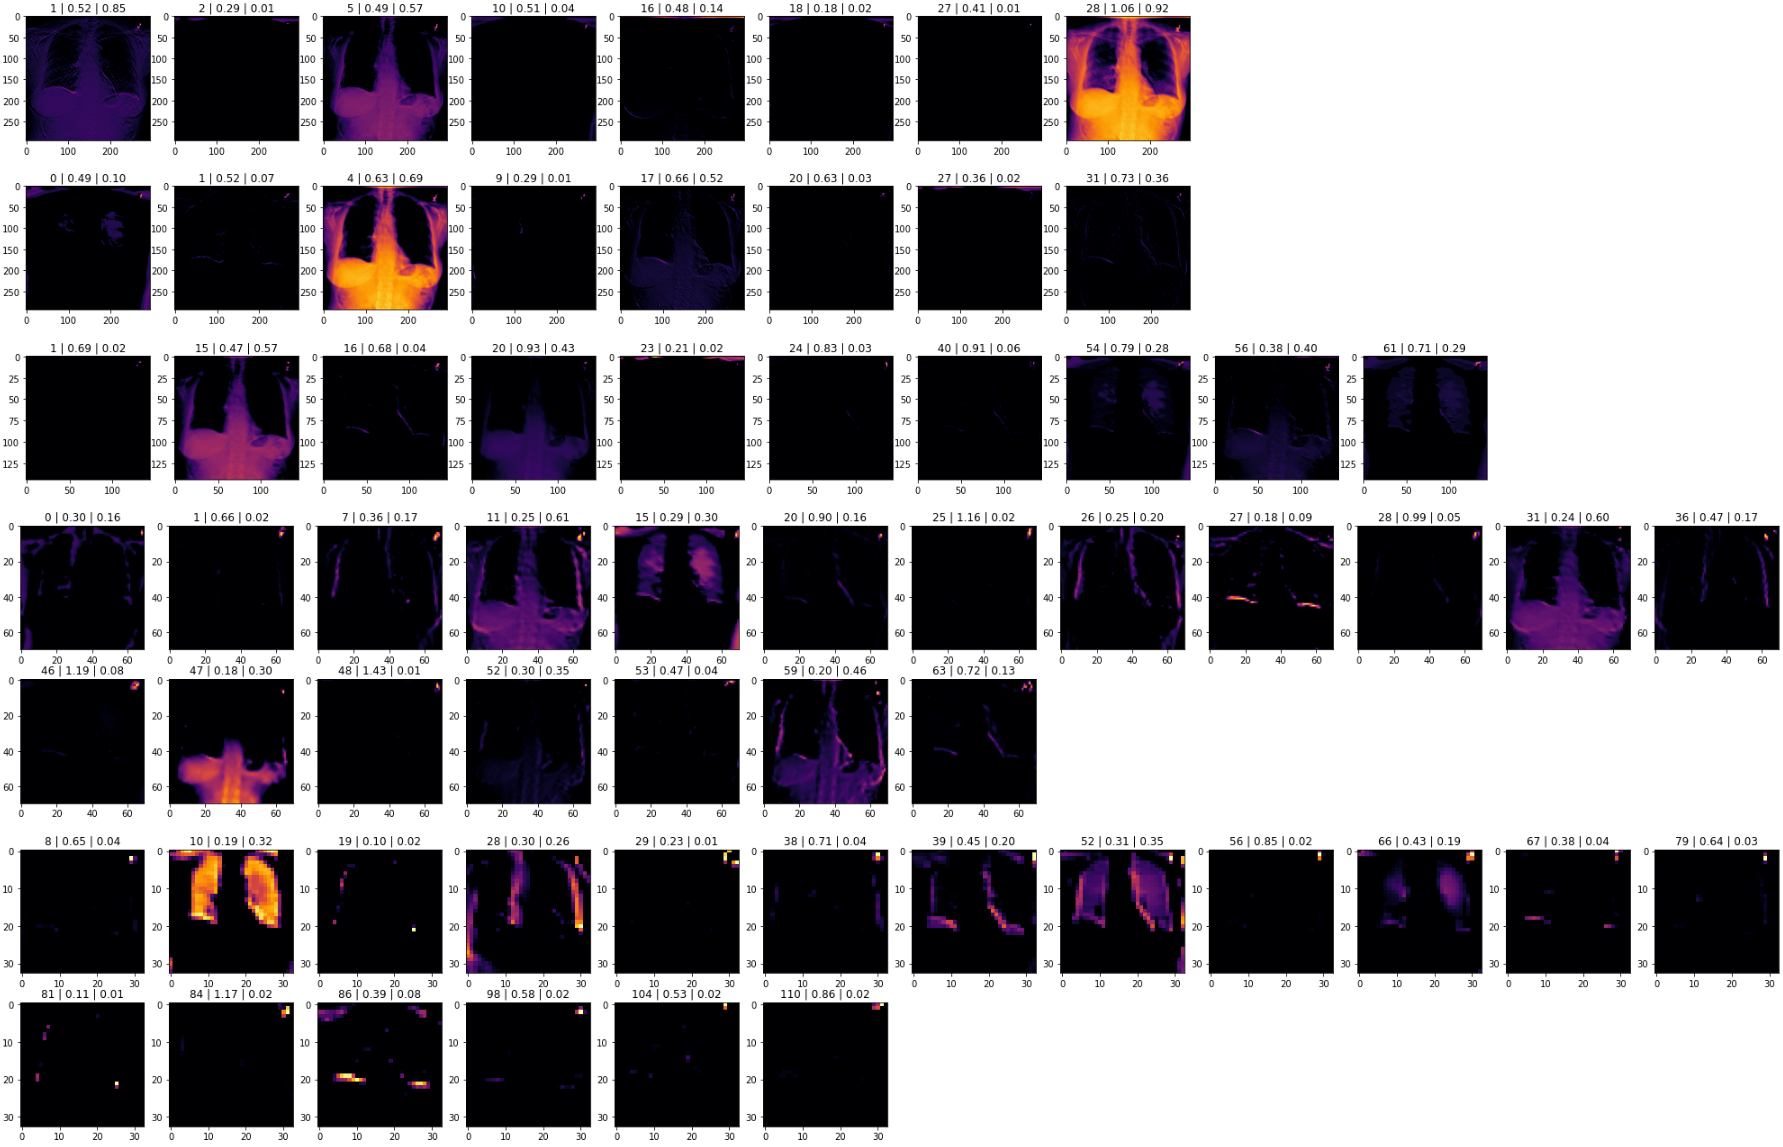
\includegraphics[width=1\textwidth,keepaspectratio=true]{normal_filters_light}
\caption{Bardziej jasne mapy cech generowane pod czas predykcji obrazu na rysunku przed poprzednim}
\label{normal_filters_light}
\end{figure}

Na rysunkach \ref{normal_filters_dark} i \ref{normal_filters_light} są wyświetlone mapy cech generowane przy predykcji choroby płuc na zdjęciu na rysunku \ref{normal_pediction}. Nad każdym obrazkiem są trzy liczby: numer filtry w danej warstwie, maksymalna wartość piksela i procent nie czarnych pikseli na danym obrazku. Są wyświetlone nie wszystkie mapy dla tego, że większość filtrów dają całkowicie czarny obrazek. Różne filtry reagują na różne kształty, dla innych zdjęć są aktywne inne filtry splotowe.

Rysunki \ref{normal_filters_dark} i \ref{normal_filters_light} są identyczne z jedną różnicą, na rysunku \ref{normal_filters_light} obrazki są bardziej jasne, żeby było lepiej widać cechę. Natomiast mapy cech na rysunku \ref{normal_filters_dark} pokazują realną jasność (siłę).

Na rysunku \ref{normal_filters_dark} bardzo dobrze widać że w ostatniej warstwie na obrazku 84 jest najjaśniejszy punkt w prawym górnym kącie. Akurat na zdjęciu w tym miejscu jest odzwierciedlona literka L. Co w teorii mówi nam że ta literka ma wielki wpływ na predykcje choroby. Co w rzeczywistości może być nie tak dla tego, że predykcja jest robiona w następnych warstwach sieci które niestety nie da się tak łatwo wyświetlić i zrozumieć. Natomiast zwiększa to szans że sieć jest wytrenowana źle albo dane są nie dobrej jakości.  


\begin{figure}[H]
	\centering
	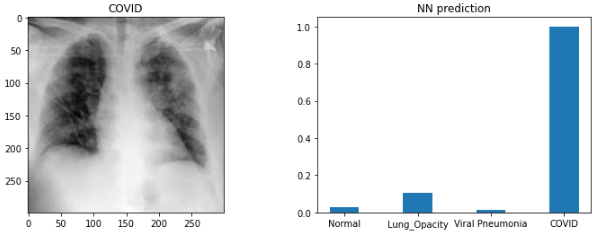
\includegraphics[width=1\textwidth,keepaspectratio=true]{covid_prediction}
	\caption{Predykcja losowego zdjęcia zdrowych płuc ze zbioru testowego.}
	\label{covid_pediction}
\end{figure}

\begin{figure}[H]
	\centering
	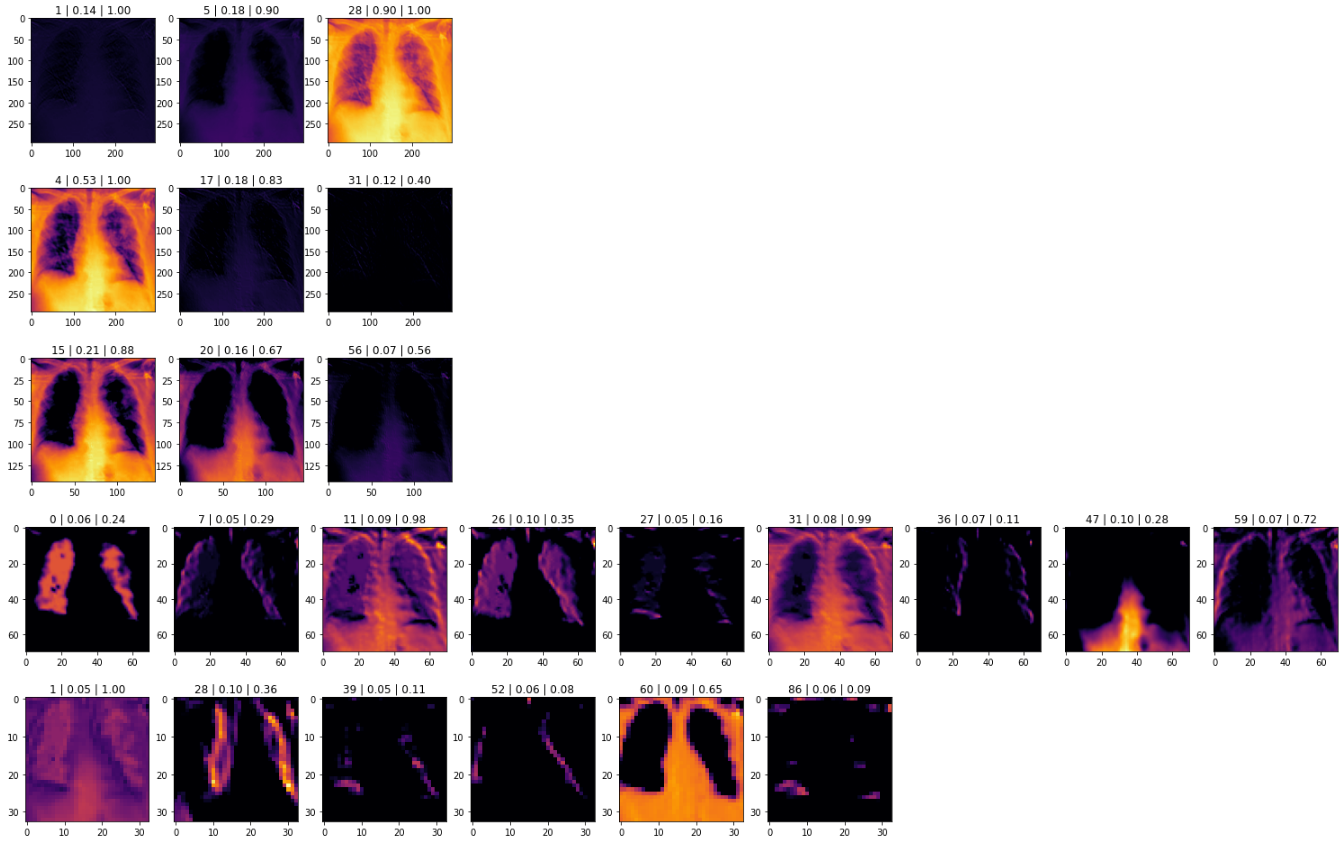
\includegraphics[width=1\textwidth,keepaspectratio=true]{covid_filters_dark}
	\caption{Mapy cech generowane pod czas predykcji obrazu na poprzednim rysunku}
	\label{covid_filters_dark}
\end{figure}

\begin{figure}[H]
	\centering
	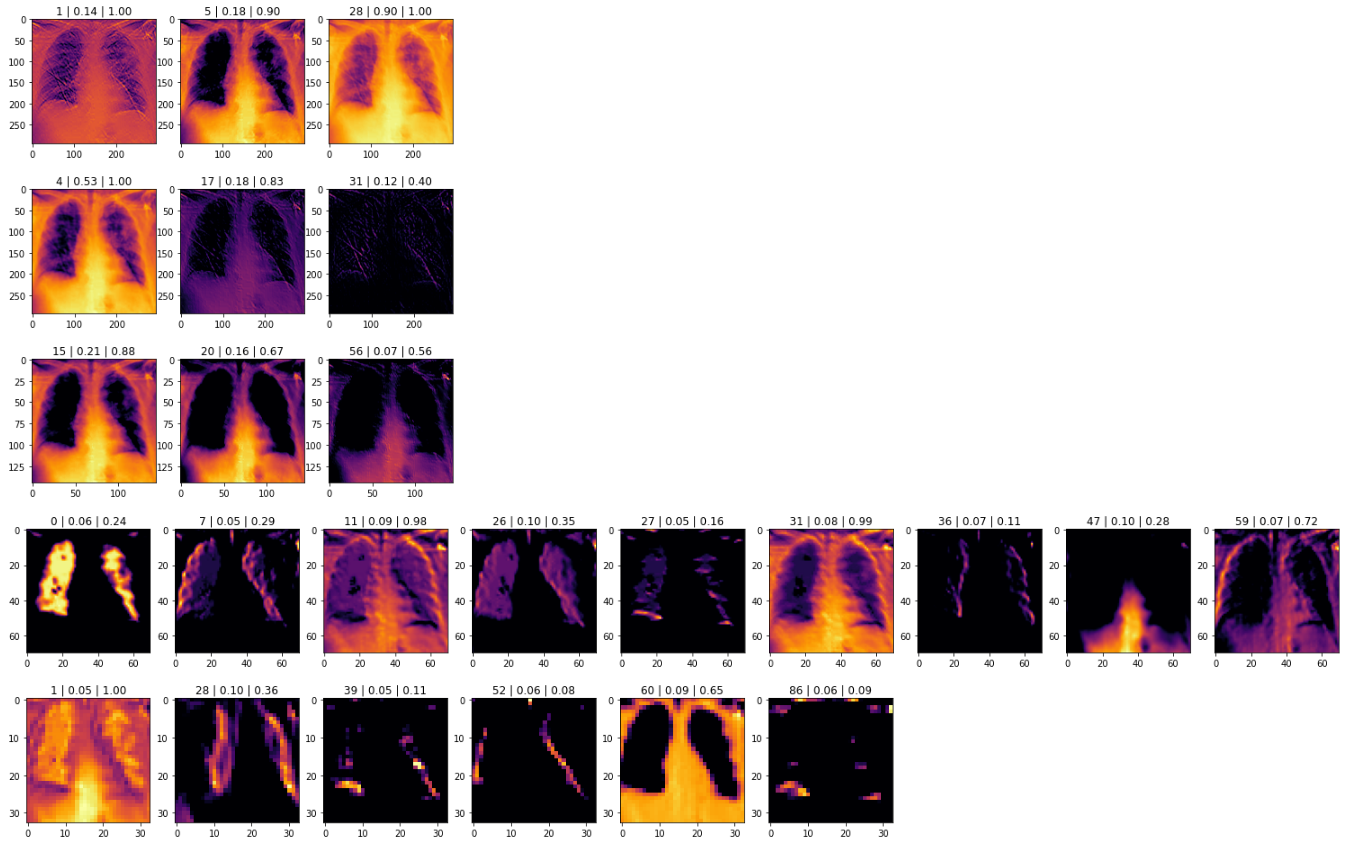
\includegraphics[width=1\textwidth,keepaspectratio=true]{covid_filters_light}
	\caption{Bardziej jasne mapy cech generowane pod czas predykcji obrazu na rysunku przed poprzednim}
	\label{covid_filters_light}
\end{figure}


Na rysunku \ref{covid_pediction} jest pokazana predykcja choroby na zdjęciu bez żadnych literek. Na rysunkach \ref{covid_filters_dark} \ref{covid_filters_light} widać że są aktywne zupełnie inne filtry oraz ilość aktywnych filtrów też jest mniejsza. Na tym przykładzie bardzo dobrze zostały wyróżnione same płuca i różne utwory wewnątrz. Nawet można uwierzyć że sieć coś "widzi" w płucach i predykcja została zrobiona na podstawie jakichś utworów wewnątrz. 

%-----------------------------------------------------------------------------------
\subsection{Statystyki używania filtrów splotowych}
Widać że dużo filtrów dają czarny obrazek i warto było sprawdzisz czy na pewno wszystkie filtry reagują na jakieś kształty. Został napisany skrypt który przeprowadza 1000 losowych obrazków ze zbioru testowego przez sieć i liczy średnie wartości otrzymanych map cech. Okazało się że nie wszystkie filtry działają poprawnie. Najprawdopodobniej jest to problem nazywany śmiercią ReLU. Neuron albo, jak w tym przypadku, cały filtr umiera kiedy zaczyna wysyłać zero bez względu na co on ma na wejściu. W przypadku kiedy neuron ma wagi które powodują że suma ważona będzie ujemna to algorytm uczenia nie jest w stanie nic zmienić, dla tego że pochodna ReLU w tym miejscu jest 0. \cite{geron}

\begin{figure}[H]
	\centering
	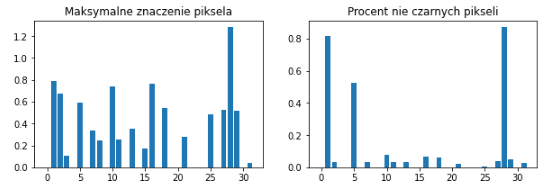
\includegraphics[width=0.8\textwidth,keepaspectratio=true]{statystyka_warstwy_1}
	\caption{Pierwsza warstwa splotowa. Działa 18 filtry z 32}
	\label{statystyka_warstwy_1}
\end{figure}

\begin{figure}[H]
	\centering
	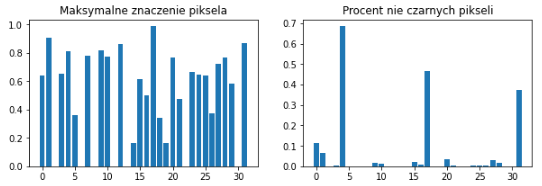
\includegraphics[width=0.8\textwidth,keepaspectratio=true]{statystyka_warstwy_2}
	\caption{Druga warstwa splotowa. Działa 25 filtry z 32}
	\label{statystyka_warstwy_2}
\end{figure}

\begin{figure}[H]
	\centering
	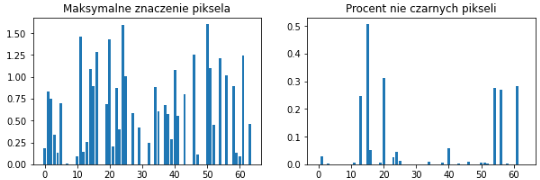
\includegraphics[width=0.8\textwidth,keepaspectratio=true]{statystyka_warstwy_3}
	\caption{Trzecia warstwa splotowa. Działa 44 filtry z 64}
	\label{statystyka_warstwy_3}
\end{figure}

\begin{figure}[H]
	\centering
	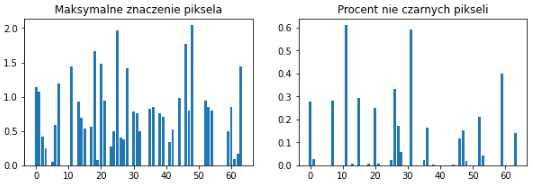
\includegraphics[width=0.8\textwidth,keepaspectratio=true]{statystyka_warstwy_4}
	\caption{Czwarta warstwa splotowa. Działa 43 filtry z 64}
	\label{statystyka_warstwy_4}
\end{figure}

\begin{figure}[H]
	\centering
	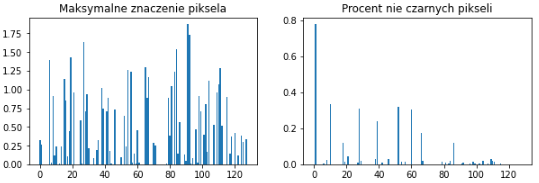
\includegraphics[width=0.8\textwidth,keepaspectratio=true]{statystyka_warstwy_5}
	\caption{Piąta warstwa splotowa. Działa 81 filtry z 128}
	\label{statystyka_warstwy_5}
\end{figure}

%-----------------------------------------------------------------------------------
\section{Eksperymenty}

%-----------------------------------------------------------------------------------
\subsection{Różne struktury sieci}
Pierwszą próbą była sieć zawierająca trzy warstwy splotowe i dwie warstwy "dense". Ta sieć miała w sobie 80,564,612 parametrów. Większą częścią tych parametrów było połączenie ostatniej warstwy splotowej i pierwszej warstwy "dense". To jest bardzo duża liczba parametrów, natomiast średni czas jednej epoki uczenia był 303 sekundy. Ten model osiągną rezultat \textit{val loss: 0.3893} i \textit{val accuracy: 0.8630}. Co jest całkiem niezły wynik. Na rysunku \ref{history_1} można zobaczyć niewielkie przetrenowanie. 

\begin{figure}[H]
	\centering
	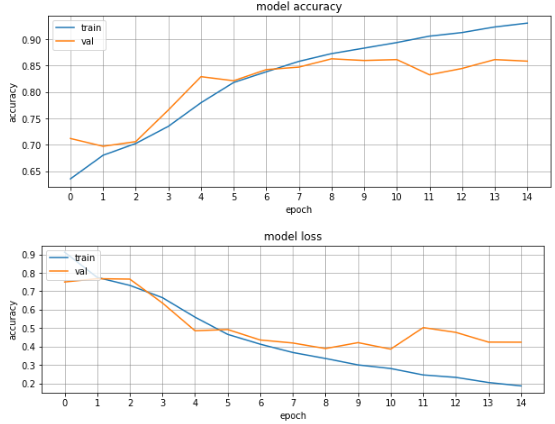
\includegraphics[width=0.8\textwidth,keepaspectratio=true]{history_1}
	\caption{Historia uczenia 1 modeli}
	\label{history_1}
\end{figure}

Drugi model miał łącznie 4,486,116 parametrów i zawierał 4 warstwy splotowe i trzy "dense". W historii uczenia tego modelu (rysunek \ref{history_2}) widać że coś poszło nie tak. Przez ostatnie cztery epoki nie było ulepszeń i uczenie zostało przerwane.

\begin{figure}[H]
	\centering
	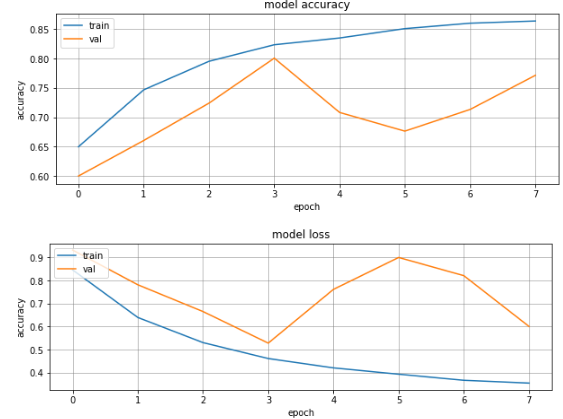
\includegraphics[width=0.8\textwidth,keepaspectratio=true]{history_2}
	\caption{Historia uczenia 2 modeli}
	\label{history_2}
\end{figure}

Trzeci model miał 4 warstwy splotowe i 3 "dense". Liczba parametrów równa się 32,157,444. To nie ulepszyło sytuacje.

\begin{figure}[H]
	\centering
	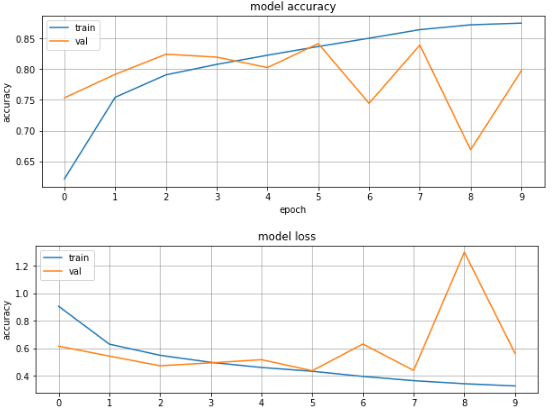
\includegraphics[width=0.8\textwidth,keepaspectratio=true]{history_3}
	\caption{Historia uczenia 3 modeli}
	\label{history_3}
\end{figure}

Czwarty raz spróbowałem wziąć najpierwszy model, dodać jedną warstwę splotowa  BatchNormalization po każdej warstwie splotowej. W teorii to miało by ulepszyć wynik i zwiększysz szybkość uczenia się. Ale niestety ani jedno ani drugie nie było fajne. Prędkość była około 345 sekund na epokę.

\begin{figure}[H]
	\centering
	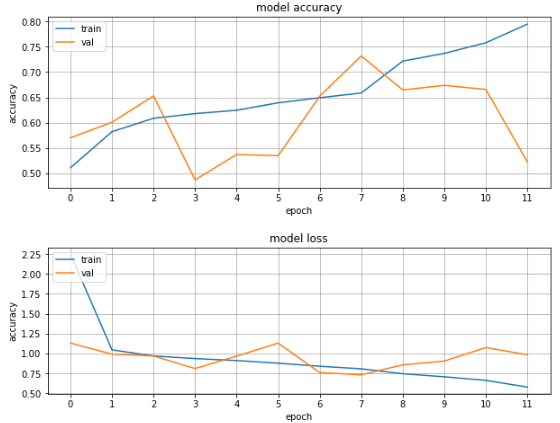
\includegraphics[width=0.8\textwidth,keepaspectratio=true]{history_4}
	\caption{Historia uczenia 4 modeli}
	\label{history_4}
\end{figure}

W piątym modelu kluczową zmianą było to że pierwsze dwie warstwy splotowe idą jedna po drugiej bez żadnej warstwy po środku. I do tego jeszcze rozmiary filtrów splotowych były po kolei 64, 64, 32, 32. Czyli odwrotnie, do tej pory robiłem rosnąco. Widać trochę przetrenowanie na końcu ale nie krytycznie. Liczba parametrów -- 20,203,396. Jest to cztery razy mniej od pierwszego modelu a rezultat jest nie gorszy.

\begin{figure}[H]
	\centering
	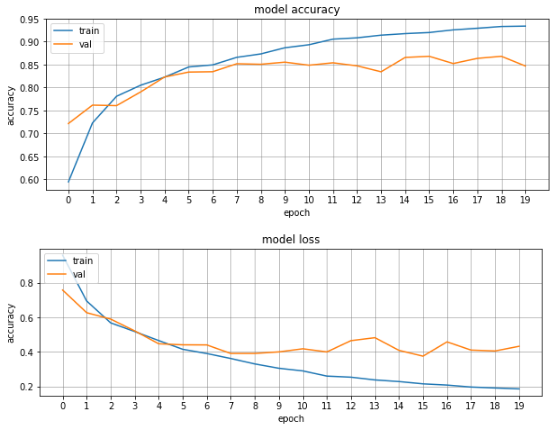
\includegraphics[width=0.8\textwidth,keepaspectratio=true]{history_5}
	\caption{Historia uczenia 5 modeli}
	\label{history_5}
\end{figure}

W szóstym i ostatnim modelu, w odróżnieniu od piątego, dodałem jedną warstwę splotową i rozmiar filtrów jest ustawiony rosnąco. Dodanie warstwy splotowej zmniejszyło wielkość ostatniej mapy cech, co zmniejsza ilość parametrów. W tym modelu jest to 16,983,268. Plus do tego to zwiększyło prędkość uczenia się, 184 sekundy na epokę. Ten model wyszedł najlepszy względem liczby parametrów i prędkością działania i też daje najlepszy rezultat, wprawie 87\% wiarygodności predykcji chorób w zbiorze testowym.  

\begin{figure}[H]
	\centering
	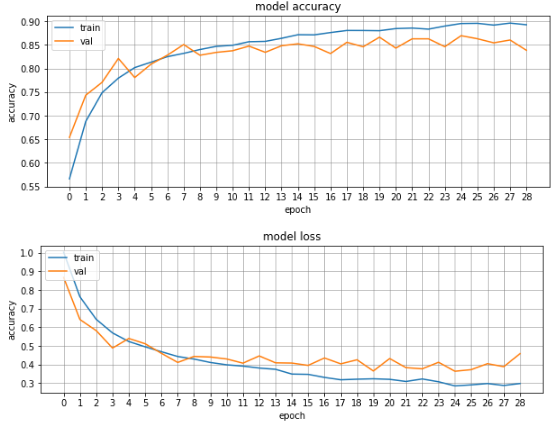
\includegraphics[width=0.8\textwidth,keepaspectratio=true]{history_6}
	\caption{Historia uczenia 6 modeli}
	\label{history_6}
\end{figure}


%-----------------------------------------------------------------------------------
\subsection{Sprawdzenie prawidłowości klasyfikacji}

Na rysunkach niżej było badane czy sieć reaguje tylko na płuca i choroby czy inne czynniki (literki, strzałki napisy...) też mają wpływ.


\begin{figure}[H]
	\centering
	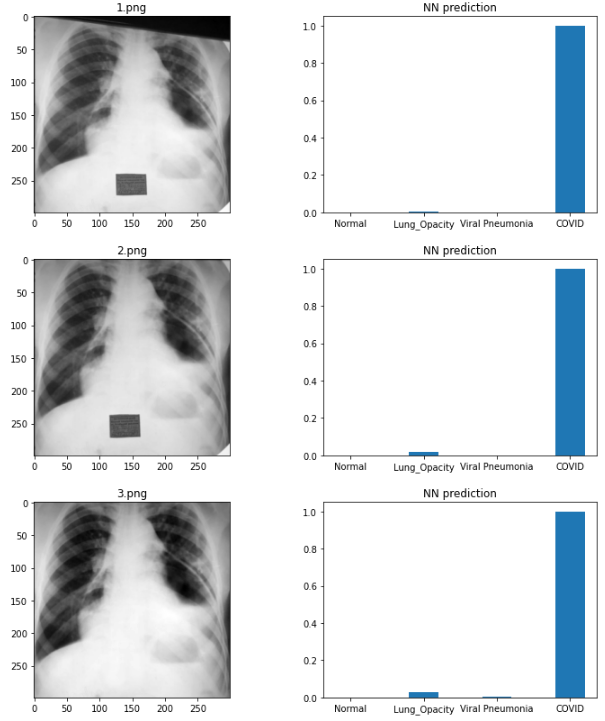
\includegraphics[width=0.8\textwidth,keepaspectratio=true]{fixing_image_exp}
	\caption{W tym przypadku wyrównanie i usunięcie karteczki na dole nie spowodowało żadnych poważnych zmian w predykcji }
	\label{}
\end{figure}

\begin{figure}[H]
	\centering
	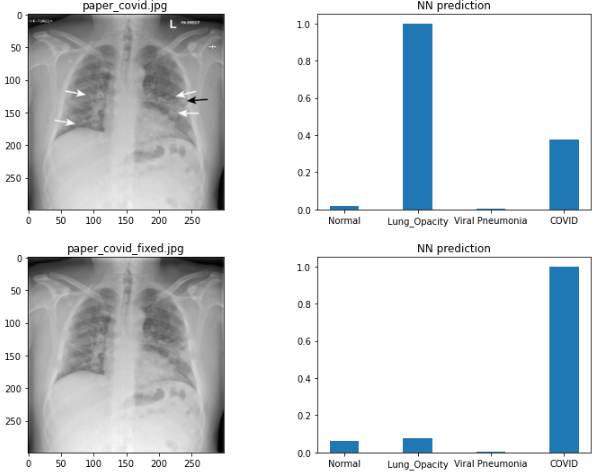
\includegraphics[width=0.8\textwidth,keepaspectratio=true]{paper_covid_exp}
	\caption{Usuniecie strzałek i literki prawym górnym rogu całkowicie zmieniły rezultat predykcji}
	\label{}
\end{figure}

\begin{figure}[H]
	\centering
	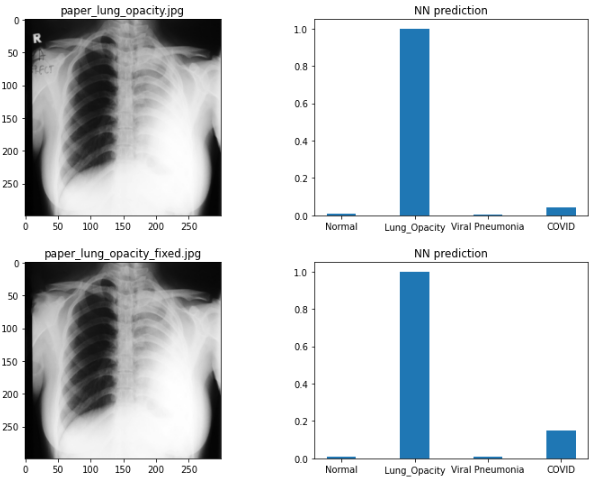
\includegraphics[width=0.8\textwidth,keepaspectratio=true]{paper_l_o_exp}
	\caption{Litera R nie wpływa na predykcje}
	\label{}
\end{figure}

\begin{figure}[H]
	\centering
	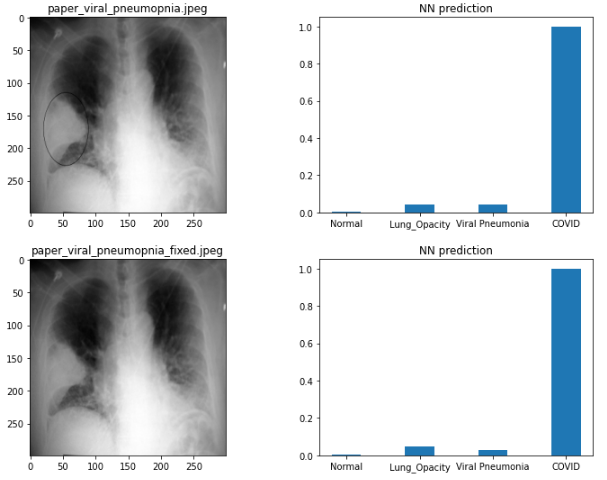
\includegraphics[width=0.8\textwidth,keepaspectratio=true]{paper_v_p_exp}
	\caption{Usuniecie koła nie powoduje zmian}
	\label{}
\end{figure}

\begin{figure}[H]
	\centering
	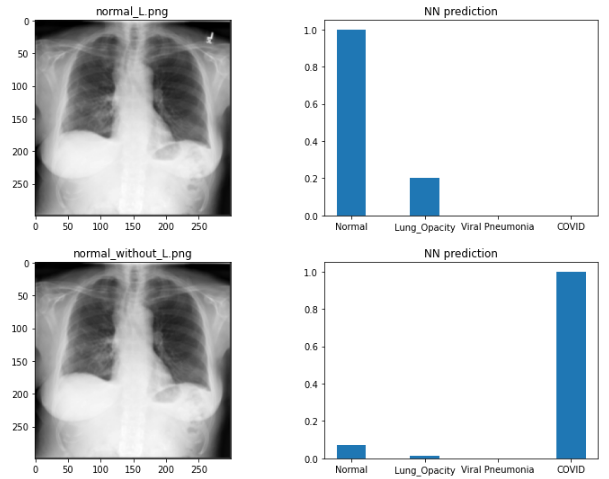
\includegraphics[width=0.8\textwidth,keepaspectratio=true]{normal_L_exp}
	\caption{Tutaj można wyciągnąć wniosek że predykcja zależy od literki w prawym górnym rogu}
	\label{}
\end{figure}

\begin{figure}[H]
	\centering
	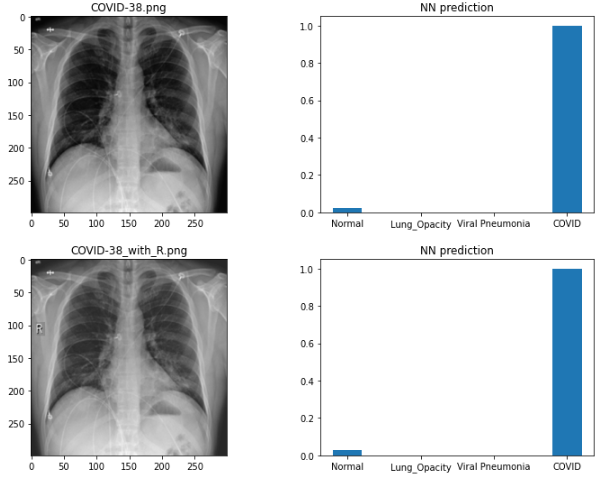
\includegraphics[width=0.8\textwidth,keepaspectratio=true]{covid_R_exp}
	\caption{Dodanie literki R(literka była wzięta ze "zdrowego" zdjęcia nie powoduje zmian)}
	\label{}
\end{figure}

\begin{figure}[H]
	\centering
	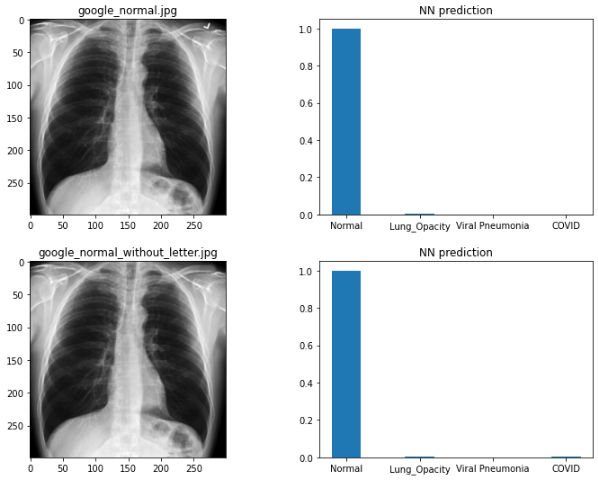
\includegraphics[width=0.8\textwidth,keepaspectratio=true]{google_normal_L_exp}
	\caption{Akurat w tym przypadku litera nie wpływa na rezultat predykcji}
	\label{}
\end{figure}



%-----------------------------------------------------------------------------------
\section{Wnioski}
Rezultat uczenia był zachęcający, w to że prawdopodobieństwo zgadywania chorób 87\% można uwierzyć. Ale jak pokazują eksperymenty i sprawdzanie, sieć czasem generuje odpowiedź na podstawie różnych literek, strzałek znajdujących się na RTG. Natomiast oczekujemy zależność predykcji od zmian płuc w odróżnieniu od zdrowych. To że na zbiorze testowym wynik jest względnie wysoki może wskazywać na złe dane treningowe i testowe. To znaczy że są jakieś zależności ukryte na podstawie których sieć i robi swoją predykcje. Można z tego wyciągnąć wniosek że sieć nauczyła się poprawnie ale dane treningowe nie są wysokiej jakości. Jako pomysł na dalszą pracę w rozwiązywaniu tego problemu można przeprowadzić wstępne przetwarzanie danych. Można by było pododawać różne losowe literki, strzałki i obiekty do zdjęć żeby nie było sensu dla sieci patrzeć na to, żeby te obiekty były szumem. Wtedy, teoretycznie, sieć mogła by więcej resursu poświadczyć na znalezienie chorób.

\bibliography{bibliografia}
	
\end{document}